% ****** Start of file apssamp.tex ******
%
%   This file is part of the APS files in the REVTeX 4.2 distribution.
%   Version 4.2a of REVTeX, December 2014
%
%   Copyright (c) 2014 The American Physical Society.
%
%   See the REVTeX 4 README file for restrictions and more information.
%
% TeX'ing this file requires that you have AMS-LaTeX 2.0 installed
% as well as the rest of the prerequisites for REVTeX 4.2
%
% See the REVTeX 4 README file
% It also requires running BibTeX. The commands are as follows:
%
%  1)  latex apssamp.tex
%  2)  bibtex apssamp
%  3)  latex apssamp.tex
%  4)  latex apssamp.tex
%
\documentclass[%
twocolumn,
%reprint,
%superscriptaddress,
%groupedaddress,
%unsortedaddress,
%runinaddress,
%frontmatterverbose, 
%preprint,
%preprintnumbers,
%nofootinbib,
%nobibnotes,
%bibnotes,
 amsmath,amssymb,
 %aps,
%pra,
prb,
%rmp,
%prstab,
%prstper,
floatfix,
]{revtex4-2}

\usepackage{graphicx}% Include figure files
\usepackage{dcolumn}% Align table columns on decimal point
\usepackage{bm}% bold math
\usepackage{chngcntr}
\usepackage{slashed}
\usepackage{amssymb}
\usepackage{wasysym}
\newcommand{\RomanNumeralCaps}[1]
    {\MakeUppercase{\romannumeral #1}}
\usepackage{float}
\usepackage{dblfloatfix}
\usepackage{blindtext}
\usepackage{longtable}
\usepackage[utf8]{inputenc}
\linespread{1.6}
%\counterwithin{figure}{section}
%\counterwithin{table}{section}
%\usepackage{hyperref}% add hypertext capabilities
%\usepackage[mathlines]{lineno}% Enable numbering of text and display math
%\linenumbers\relax % Commence numbering lines

%\usepackage[showframe,%Uncomment any one of the following lines to test 
%%scale=0.7, marginratio={1:1, 2:3}, ignoreall,% default settings
%%text={7in,10in},centering,
%%margin=1.5in,
%%total={6.5in,8.75in}, top=1.2in, left=0.9in, includefoot,
%%height=10in,a5paper,hmargin={3cm,0.8in},
%]{geometry}

\begin{document}

\preprint{APS/123-QED}

\title{Long-lived Particles (LLPs) in the SM and BSM extensions}% Force line breaks with \\
%\thanks{A footnote to the article title}%

\author{Kai Wei}
\affiliation{%
 Department of Physics, The Ohio State University
}%


\date{\today}% It is always \today, today,
             %  but any date may be explicitly specified

\begin{abstract}
In both Standard Model (SM) and Beyond Standard Model (BSM) extensions, particles with long lifetime are 
\end{abstract}

%\keywords{Suggested keywords}%Use showkeys class option if keyword
                              %display desired
\maketitle

%\tableofcontents

% Insert Introduction
\section{Introduction}
[Introduction of LLPs, explain what LLP is, why it is important in BSM searching, signature in collider experiments, current status of LLP search in various experiments]

Long-lived particles (LLPs) are particles with lifetime comparable to particles at weak scale in Standard Model (SM). LLPs exist in Standard Model and commonly predicted in beyond Standard Model (BSM) physics. 

The long lifetime can arise from multiple reasons, including approximate symmetries that stabilize the LLPs, small coupling which narrow the decay widths of LLPs, and suppressed phase space for final state \cite{alimena2019searching}. In some cases, more than one reason can combine and lead to long lifetime in both SM and BSM. Since the proper decay lengths,$c\tau$, of LLP is comparable to the size of detector, the signatures are exotic in collider physics and distinguishable between SM and BSM. For the above properties, experimental signatures of LLPs in LHC are good probe for the search of new physics (NP) while are varied and complex. For example, LLPs signatures can include disappearing, appearing, and kinked tracks, displaced vertices and jets in inner detector, calorimeter, and muon system region, as well as trackless localized energy deposits in calorimeters. The behaviors of LLP signatures are summarized in Fig.\ref{fig:LLPsignature}

\begin{figure}[!h]
    \centering
    \caption{Schematic of the variety of challenging, atypical experimental signatures that can result from BSM LLPs in the detectors at the LHC. Shown is a cross-sectional plane in azimuthal angle, $\phi$, of a general purpose detector such as ATLAS or CMS. From \cite{russell2017llp}}
    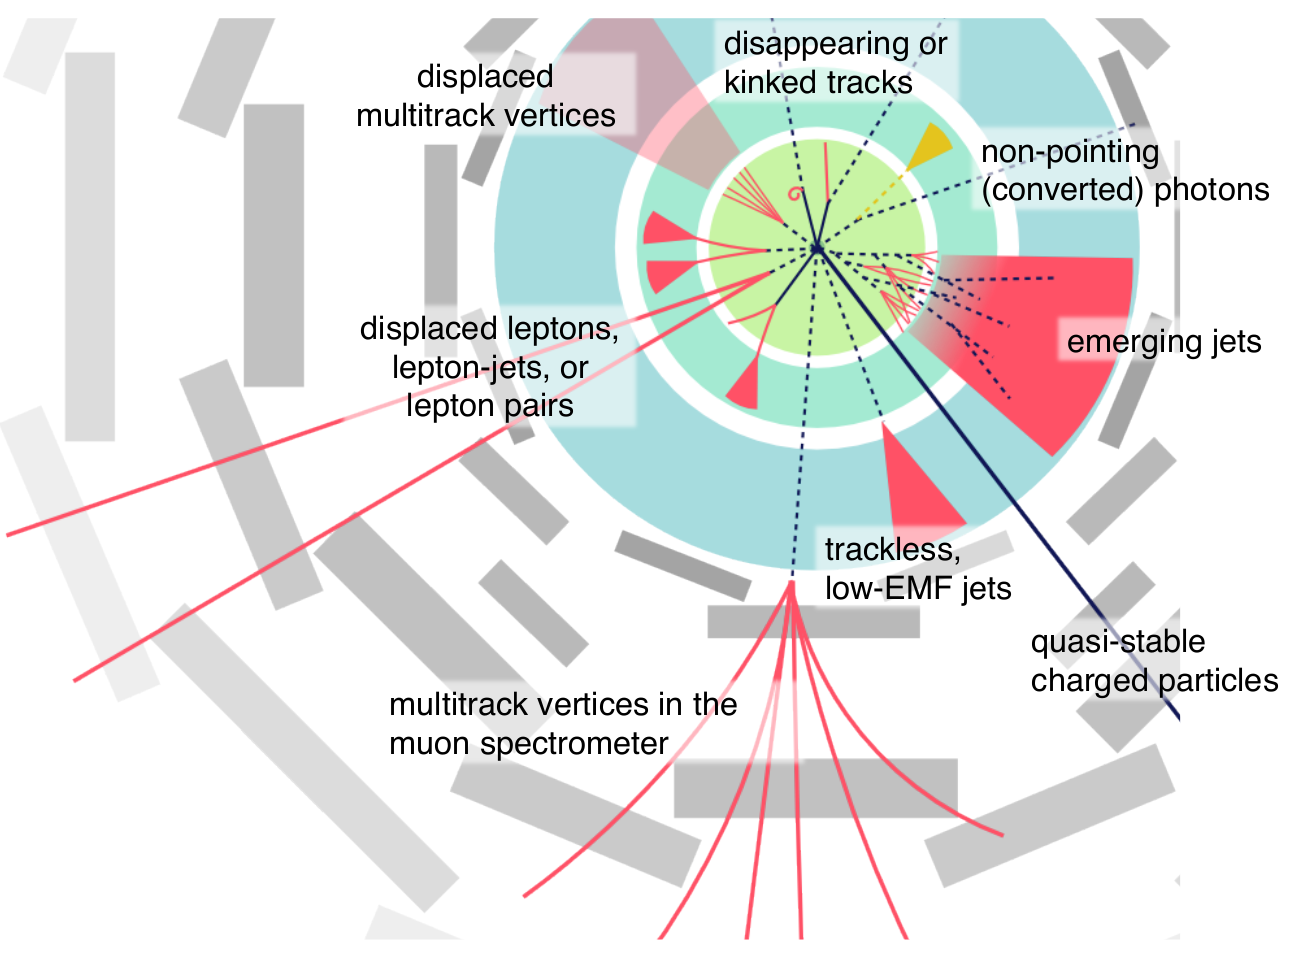
\includegraphics[width=0.5\textwidth]{fig/LLPSignature.png}
    \label{fig:LLPsignature}
\end{figure}

Although the LLP signatures are distinguishable from SM signatures, standard reconstruction algorithm developed for SM process may reject events with LLP signatures due to their unusual behaviors and dedicated analysis are necessary. These signatures also resemble background including detector noise, pile-up particles, and mis-reconstructed objects which is inaccurate in  Monte Carlo (MC) simulation. It is a challenge to model all sources of background and  make precise estimation in LLP searches. Furthermore, triggers and algorithms optimized for LLP signatures should be applied to simplify searches in future.

Heretofore, many searches for LLPs have been performed at the Large Hadron Collider (LHC). Detailed searches are described in Chapter IV. Existing LLP searches prove the necessity of methods for identifying signals of LLP and vetoing backgrounds. 

% Insert Theoretical Motivation
\section{Theoretical Motivation}
Since the lifetimes of particles in the SM cover an enormous range of magnitude, a variety of particles in the SM are long-lived particles. From the aspect of experiment, the signature of long-lived particles in the SM are well-understood and can be easily removed from signatures searching for new physics. While some similar mechanism  shared by long-lived particles in both SM and BSM. 

In SM, there are several ways to prolong the lifetimes of particles. The first way is off-shell mediator. In the standard model, quark flavor is conserved by all but weak interaction while the decay is highly off-shell due to the large mass of $Z/W$. A example is the decay of charged pion $\pi^{\pm}$, made up with up and down quark, it decays via weak interaction and $m_{W^{\pm}} >> m_{\pi^{\pm}}$, and the decay width scales as 
\begin{equation}
   \Gamma_{\pi^{\pm}} \sim g_{W}^4 (\frac{m_{\pi}}{m_W})^{4} m_{\pi}
\end{equation}

\textbf{Need check}. A second way is nearly mass degeneration which lead to suppressed final-state phase space. In neutron decay $ n^0 \rightarrow p^+ + e^- + \bar{\nu_{e}}$, the mass split between neutron and proton is tiny  due to the isospin symmetry which broken by the masses of quarks and electromagnetic interaction. The neutron decay then also suppressed by off-shell $W^-$. And a third way is small coupling,  a dummy example in SM is flavour-changing neutral currents $\mu \rightarrow e \gamma $ where the coupling is suppressed by tiny neutrino Yukawa couplings \textbf{check with Stuart}. 

With a survey of BSM extensions, LLPs are commonly predicted in a variety of theories that address fundamental mysteries in particle physics such as naturalness, baryogenesis, non-zero neutrino masses and dark matter.

For naturalness problem, Supersymmetry (SUSY) is a well-known solution of the hierarchy problem of higgs mass. Within Minimal Supersymmetric Standard Model (MSSM), Anomaly-mediated supersymmetry breaking (AMSB) predicts a particle mass spectrum in which a small mass splitting exist. The mass splitting can be small as several MeV which compress final-state phase space and allow  macroscopic lifetime. Another case is  Gauge Mediated SUSY breaking(GMSB) with the scale of SUSY breaking $\sqrt{F}$, where the gravitino is the lightest supersymmetric particle (LSP) whose mass scales as 
\begin{equation}
    m_{3/2} \sim \frac{F}{M_{pl}}
\end{equation}
and the coupling of the next-to-lightest supersymmetric particle (NLSP) to LSP scales as $1/F$. There is a range of $F$ where the coupling is sufficiently small and NLSP has macroscopic lifetime. For non-minimal SUSY model, R-parity violating (RPV) interaction is considered given null results for LPC SUSY searches \textbf{[cite]}. Low-energy results have constrained flavor violation interaction significantly \textbf{[cite]} and the LSP which decays into SM particles through RPV interaction should be long-lived particle. 

\iffalse
In the QCD sector, another naturalness concern is the Strong CP problem \textbf{[cite]}, the gauge invariance allows CP-odd term: 
\begin{equation}
    \mathcal{L}_{\theta} = \theta \frac{g^{2}_{S}}{32\pi^{2}}G^{a}_{\mu\nu}\tilde{G}^{\mu\nu}_{a}
\end{equation}
while $\theta$ is a dimensionless parameter. The actual value of $\theta$ is extremely close to zero, $|\theta|< 10^{-10}$, with measurements of nucleon electric dipole moments. By introducing an axion which is a Goldstone boson of a QCD-anomalous Peccei-Quinn (PQ) symmetry \textbf{[cite]}, small $\theta$ value can be explained.
\fi

Baryongenesis is another puzzle which is important for the understanding of early-age universe. Evidences indicate that the observable universe originates from a compressed dense state that filled with a hot primordial plasma and still expanding. If assuming the amounts of matter and anti-matter were exactly the same during that epoch, they would have annihilated as the universe cooled down and no baryons would be left to form galaxies. Hence, the presence of baryons indicates there is asymmetry between matter and anti-matter. The magnitude of \textit{baryon asymmetry of the universe} (BAU) can be estimated by cosmological measurement of baryon to photon ratio, or equivalently the ratio $Y_B = (n_B-n_{\barB})/s$ where $n_B-n_{\barB}$ is the comoving baryon density and $s$ is the entropy density. The value of $Y_B$ can be extracted from both the Cosmic Microwave Background (CMB) anisotropy power spectrum and the abundance of light elements in the intergalactic medium. 

% Insert Detector description
\section{The CMS detector}
The overall layout of CMS is shown in \ref{fig:CMSdetector}.
At the heart of CMS apparatus sites a 4$T$ superconducting solenoid with 5.9m inner diameter. The tracker system and the calorimeters locate inside the solenoid volume which provide good momentum and energy resolution for both charged and neutral particles as well as particle identification (PID) power. The return field of superconducting solenoid is strong enough to saturate 1.5m of iron and cover the whole muon system.

\begin{figure}
    \centering
    \caption{An exploded view of the CMS detector. From Ref. \cite{cmstdr}}
    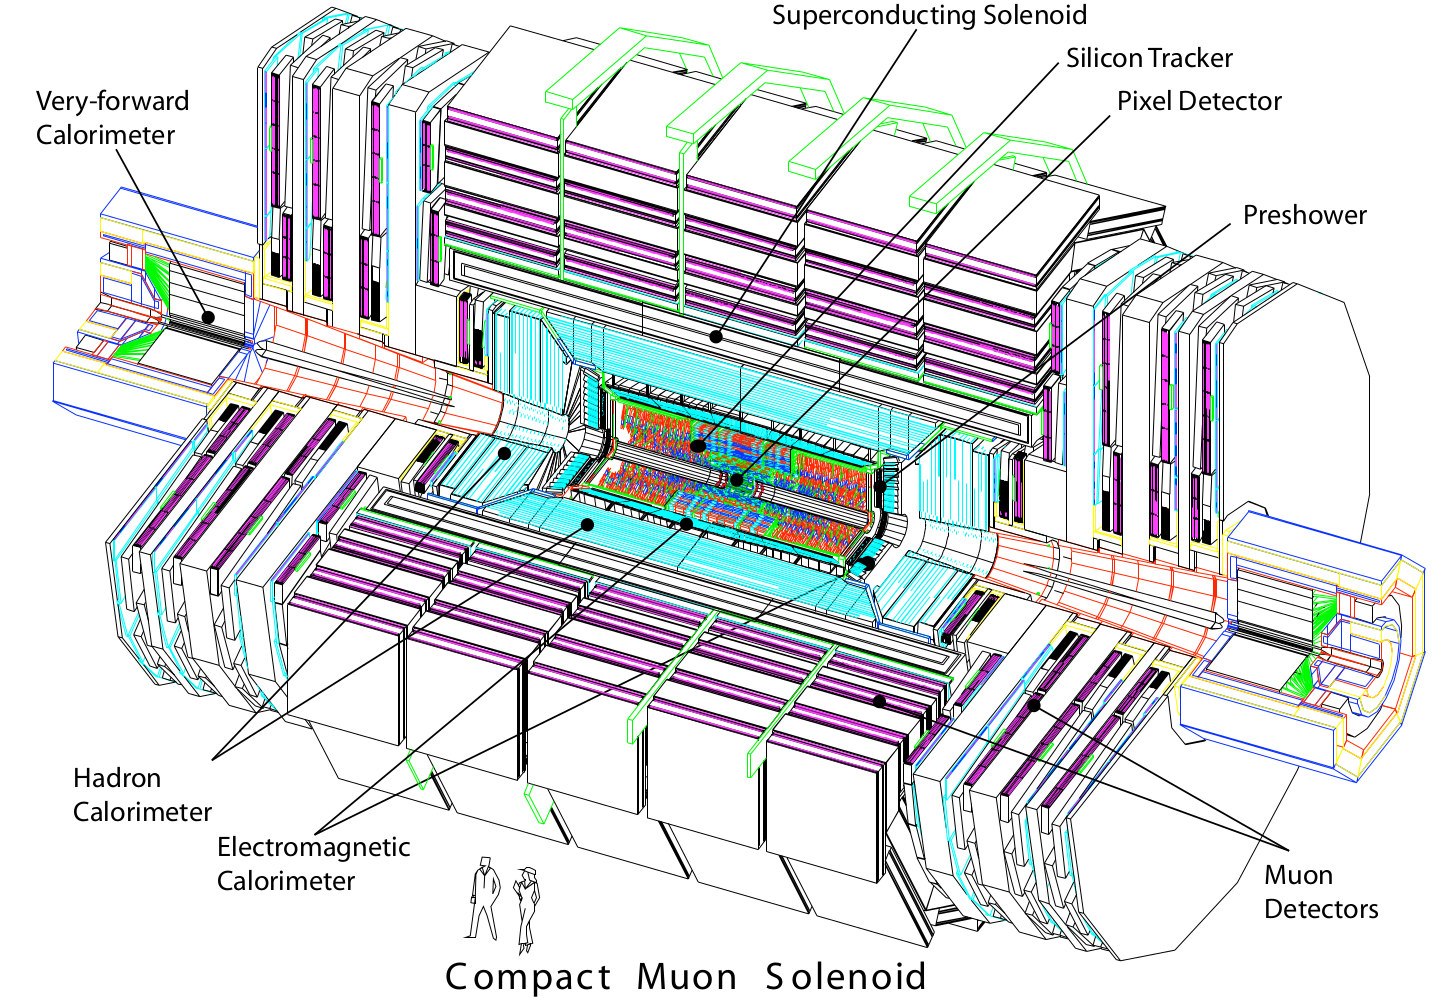
\includegraphics[width=0.5\textwidth]{fig/CMSdetector.png}
    \label{fig:CMSdetector}
\end{figure}

The magnetic field in CMS is generated by a superconducting solenoid which provides strong bending power and momentum resolution of $\Delta p/p \approx 10\% $ at $p=1TeV/c$. The parameters of the superconducting solenoid are listed in Tab.\ref{tab:magnet_parameters}:

\begin{table}[!h]
    \centering
    \caption{Parameters of the CMS superconducting solenoid. From Ref.\cite{cmstdr}}
    \begin{tabular}{|l|c|}
    \hline
    Field          &   4T      \\
    \hline
    Inner Bore     &   5.9m    \\
    \hline
    Length         &   12.9m   \\
    \hline
    Number of Turns & 2168     \\
    \hline
    Current         & 19.5kA   \\
    \hline
    Stored energy   & 2.7GJ    \\
    \hline
    Hoop stress     & 64 atm     \\
    \hline
    \end{tabular}
    \label{tab:magnet_parameters}
\end{table}

The inner tracker system is composed of silicon pixel modules placed close to the interaction region. The inner tracker is designed for high luminosity and large track multiplicities. The pixel detector are placed close to the interaction region to improve the measurement of the impact parameter as well as the position of secondary vertices. Thin silicon sensors of thickness $100-150\mu m$ are segmented into pixel size of $25 \times 100 \mu m^2$ or $50 \times 50 \mu m^2$ which provide enough radiation tolerance and deliver the desired performance in term of detector resolution, occupancy, and two-track separation. As shown in Fig. \ref{fig:tracker}, the inner tracker is composed of 4 cylindrical layers in barrel region and 8 small plus 4 large disc layers in end-cap region. The acceptance extends to  $|\eta| \approx 4$. 

The outer tracker is composed of six cylindrical barrel layers of silicon microstrip detector in the central region, covering the region of $|z|<1200mm$, complemented on each forward side by five endcap double-discs in the region of $1200 < |z| < 2700mm$. The silicon microstrip detectors provide the required granularity and precision. Modules are installed between $r \approx 21cm$ and $r \approx 112cm$. 

\begin{figure}[!h]
    \centering
    \caption{Sketch of one quarter of the tracker layout in r-z view. In the Inner Tracker the green lines correspond to pixel modules made of two readout chips and the yellow lines to pixel modules with four readout chips. In the Outer Tracker the blue and red lines represent the two types of modules described in the text. From Ref.\cite{collaboration2017phase}}
    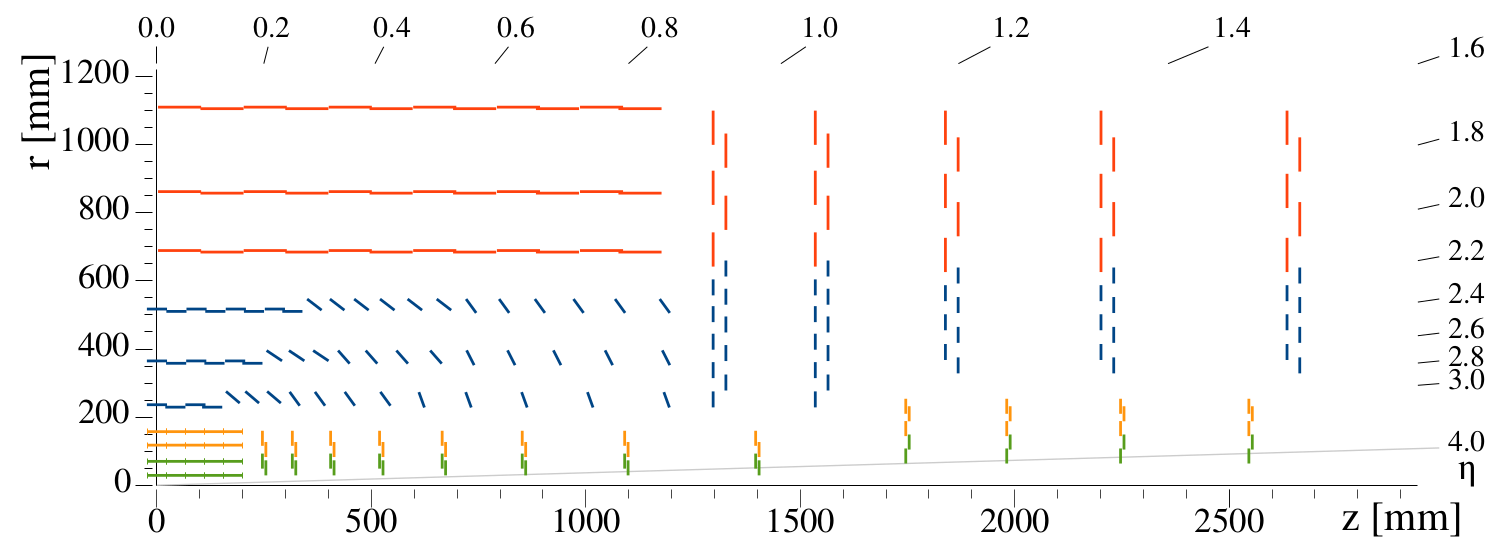
\includegraphics[width=0.5\textwidth]{fig/tracker.png}
    \label{fig:tracker}
\end{figure}

The EM calorimeter (ECAL) uses lead tungstate ($PbWO_4$) crystals with coverage in pseudorapidity up to $|\eta| < 3.0$. These crystals have short radiation ($X_0$ = 0.89 cm) and Moliere (2.2cm) lengths, short photon emission time ($80\%$ of the light is emitted within 25 ns) and radiation hard (up to 10 Mrad). The scintillation light is detected by silicon avalanche photodiodes (APDs) in the barrel region and vacuum phototriodes (VPTs) in the endcap region. The ECAL contains a barrel region and endcap region, corresponding to $0 < |\eta| < 1.479$ and $1.479 < |\eta| < 3.0$ accordingly. The crystals in the barrel section (EB) have a length of 230 mm, corresponding to 25.8 $X_0$, while the ones in the endcaps (EE) have a length of 220 mm (24.7 $X_0$). The energy resolution of ECAL can be parameterized as a function of energy: 

\begin{equation}
    (\frac{\sigma}{E})^2 = (\frac{S}{\sqrt{E}})^2 + (\frac{N}{E})^2 + C^2
\end{equation}

where $S$ is the stochastic term term, $N$ is the noise and the $C$ the constant. The values of these parameters are listed in the figure.

\begin{figure}[!h]
    \centering
    \caption{ECAL supermodule energy resolution, $\sigma_E/E$, as a function of electron energy as measured from a beam test. From Ref.\cite{cmstdr}}
    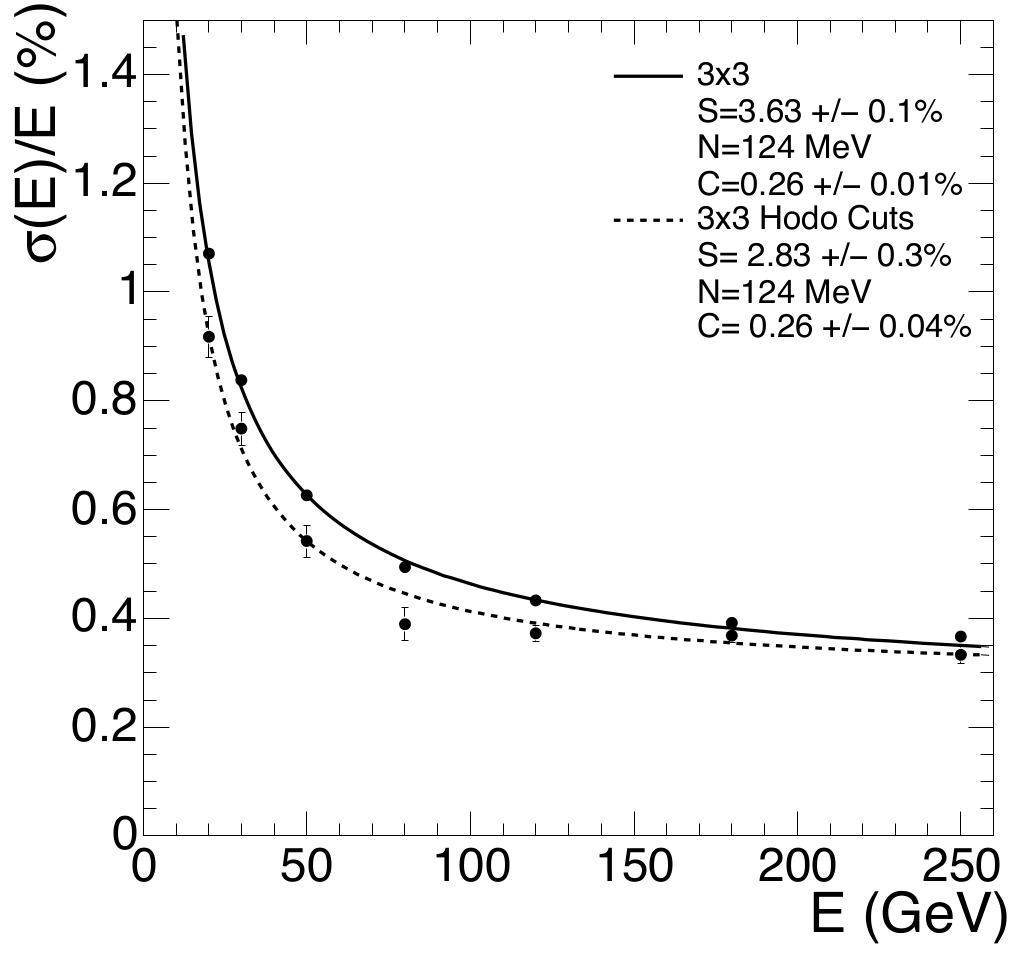
\includegraphics[width=0.45\textwidth]{fig/energyresolution.png}
    \label{fig:energyresolution}
\end{figure}

The ECAL is surrounded by a brass/scintillator sampling hadron calorimeter (HCAL) with coverage up to $|\eta | < 3.0$. The scintillation light converted by wavelength-shifting (WLS) fibres embedded in the scintillator tiles and channeled to photodetectors via clear fibres. The photons are detected by hybrid photodiodes (HPDs) that can provide gain and operate in high axial magnetic fields. The central calorimetery is complemented by a "tail-catcher" in the barrel region which extend the material length to 11 hadronic interaction length $\lambda_I$. The thickness in interaction lengths varis from $7-11 \lambda_I$ for HCAL depending on $\eta$. Coverage between pseudorapidities of 3.0 and 5.0 is provided by the steel/quartz fibre Hadron Forward (HF) 

The muon system (MS) containing 4 muon "stations". The layout of muon system is shown in fig. \ref{fig:muonsystem} Each station consists of several layers of aluminum drift tubes (DT) in the barrel region and cathode strip chambers (CSCs) in the endcap region, complemented by resistive plate chambers (RPCs) in  both region. In the barrel region ($|\eta| < 1.2$), where the muon rate is low and the residual magnetic field in the chambers is low, DT chambers are used. In endcap region, where the muon rate and magnetic field are high, CSC are deployed and cover the region up to $|\eta| < 2.4$.

\begin{figure}[!h]
    \centering
    \caption{Layout of one quarter of the CMS muon system for initial low luminosity running. THe RPC system is limited to $|\eta| < 1.6$ in the endcap, and for the CSC system only the inner ring of the ME4 chambers have been deployed. From Ref.\cite{cmstdr}}
    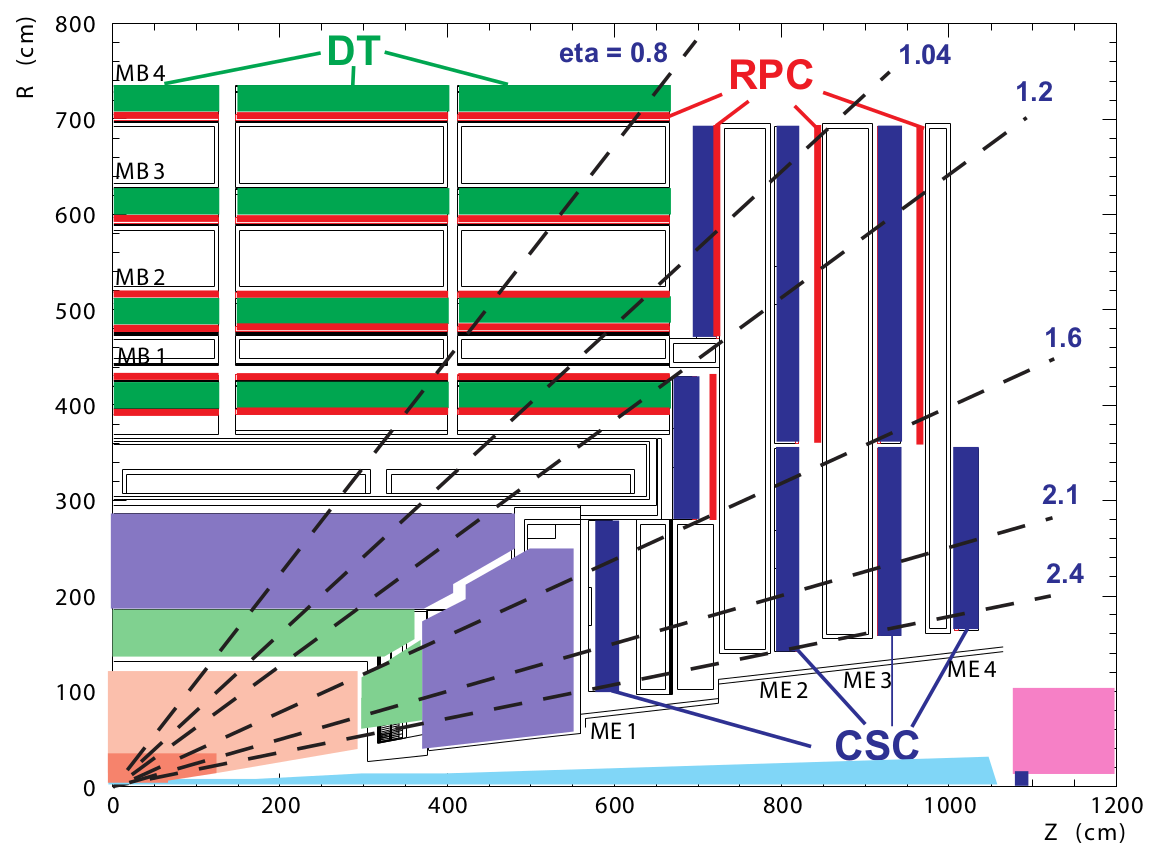
\includegraphics[width=0.5\textwidth]{fig/muonsystem.png}
    \label{fig:muonsystem}
\end{figure}

The CMS trigger and data acquisition system consists 4 parts: the detector electronics, the Level-1 (L1) trigger processors, the readout network, and an online event filter system for High-Level Trigger (HLT). The L1 triggers contains the calorimetry and muon system as well as some correlation of information between systems. The L1 decision is based on the presence of "trigger primitive" objects e.g. photons, electrons, muons and jets passing $E_T$ or $p_T$ thresholds. Reduced-granularity and reduced-resolution data are used to reconstruct trigger objects. Global sum of $E_T$ and $E_T^{miss}$ are also employed for global trigger.  The design value of L1 rate is 100 kHz by the average time to transfer full detector information through the readout system. The event selection at the HLT using reconstructed objects and identification criteria to select events with possible interest for data analysis. The HLT hardware consists of the event filter farm (EVF) composed of commodity computer. The filtering process uses the full precision of the data from the detector, and the selection is based on offline-quality reconstruction algorithms. The data processing of the HLT is structured around the concept of a HLT path, which is a set of algorithmic processing steps run in a predefined order that both reconstructs physics objects and makes selections on these objects. HLT reduce the the L1 output rate of 100 kHz to order of 1kHz for massive storage.

A more detailed description of the CMS detector can be found in  \cite{adolphi2008cms}


% Insert Current Collider Experiments for LLP
\section{Experimental coverage of Long-lived Particle Signature in Collider Experiments}

There are a broad variety of signatures of LLPs in collider experiments as shown in introduction. It is challenging to make a full coverage of experimental signatures for all possible LLP decay processes with the varied and atypical objects in LLP searches. To comprehensively review current experimental coverage, searches are classified into different channels, including hadronic decays, leptonic decays, semi-leptonic decays, photonic decays and exotic signatures. The displaced lengths also affect the signature and methods of LLP researches. LLP signature in collider experiments can be categorized into the Cartesian product of decay channels and decay positions. For many LLP signatures, a major challenge is the lack of efficient trigger. With the exception of certain dedicated triggers on ATLAS, no L1 trigger are currently available exploiting the displaced nature of LLP signatures. Current constraints on LLPs, algorithms optimized for displaced algorithm as well as trigger strategies on collider experiments are reviewed.
\iffalse
%\onecolumngrid
\begin{table*}[!htbp]
    \centering
    \caption{LLP signatures are categorized into (decay channel)$\times$(displaced length).}
    \begin{tabular}{|p{2.5cm}|p{2.5cm}|p{2.5cm}|p{2.5cm}|p{2.5cm}|p{2.5cm}|}
        \hline
                        & \textbf{hardonic}  & \textbf{leptonic} & \textbf{semi-leptonic} & \textbf{photonic} & \textbf{exotic}    \\
        \hline
        \textbf{Tracker}    & displaced jets (+ $\slashed{E}_T$) & displaced lepton & & &            \\
        \hline
        \textbf{ECal/HCal}  &    & & & &           \\
        \hline
        \textbf{MS}         &     & & & &          \\
        \hline
        \textbf{Beyond MS}  &     & & & &          \\
        \hline
        \end{tabular}
    \label{tab:LLPsignature}
\end{table*}
%\twocolumngrid
\fi

\subsection{Hadronic Decays}
Several researches are performed on ATLAS and CMS, including searches for two objects decaying in HCAL \cite{Aaboud:2019opc,Aad:2015asa}, ID/MS \cite{Aad:2015uaa,Aaboud:2018aqj} and ID decays with large $\slashed{E}_T$ ( +jets/leptons) \cite{Aaboud:2017iio,Aad:2015rba} , displaced jets \cite{Sirunyan:2018vlw,Sirunyan:2017jdo,CMS:2014wda} and displaced vertices (DV) in multijet events \cite{Sirunyan:2018pwn}. 

\subsubsection{hadronic decays in ATLAS}
The reconstruction of displaced track is an essential part of displaced object identification. In the ATLAS ID, displaced track reconstruction follows a two-step procedure. In the first iteration, the default track identification algorithm is applied. Hits which are not associated to track in the first run are used in a second run with loose requirements on the transverse and longitudinal impact parameter ($d_0$ and $z_0$) and number of silicon hits shared with other tracks. This algorithm is referred to as \textit{large radius tracking} (LRT) algorithm by ATLAS collaboration. 
Dedicated \textit{CalRatio} and \textit{MuonRoI} triggers are employed for LLP decaying in the HCAL/MS \cite{Aaboud:2019opc,Aaboud:2017iio}. For hadronic decay of neutral particle into two  in calorimeter, a higher ratio of energy deposit in HCAL is expected while there is no associated track to the energy deposit. The ratio $E_H/E_EM$, referred as \textit{CalRatio} is adopted as a dedicated trigger for neutral LLPs decaying near the outer layers of ECAL or within the HCAL. For hadronic decay in ATLAS muon spectrometer, the Muon RoI Cluster trigger which requires a $\Delta R=0.4$ radius regions in MS barrel/endcap containing 3/4 muon RoIs \cite{Aad:2013txa} are used for decays of LLPs in MS, the \textit{MuonRoI} trigger is efficient for LLPs decays between $3-7 m$ transversely or $5-13 m$ longitudinally from the primary vertex (PV), for LLP masses greater than $10 GeV$. A combined result of neutral decay in calorimeter and muon spectrometer is shown in Fig.\ref{fig:NeutralLLPinATLAScalSummary}. The combined result shows good sensitivity for $c\tau \sim 1m$ which decided by trigger strategy and the geometry of ATLAS detector.
\begin{figure}[!htbp]
    \centering
    \caption{The combined limits for models with $m_\Phi = 125 GeV$ and $m_\Phi = 600 GeV$ from the \textit{CalRatio} and \textit{MuonRoI} analysis with process $\Phi \rightarrow ss \rightarrow fff^{'}f^{'}$, which separated into the MS 1-vertex plus $E_T^{miss}$ (MS1) and MS 2-vertex (MS2) components. The MS1 component of the MS displaced jet search was only applied to models with $m_\Phi = 125 GeV$. The expected limit is shown as a dashed line with shading for the $\pm 1\sigma$ band, while the observed is a solid line. The colours of the shading and solid and dashed lines refer to the limits from each analysis and their combination, as indicated in the legend. From Ref.\cite{Aaboud:2019opc} }
    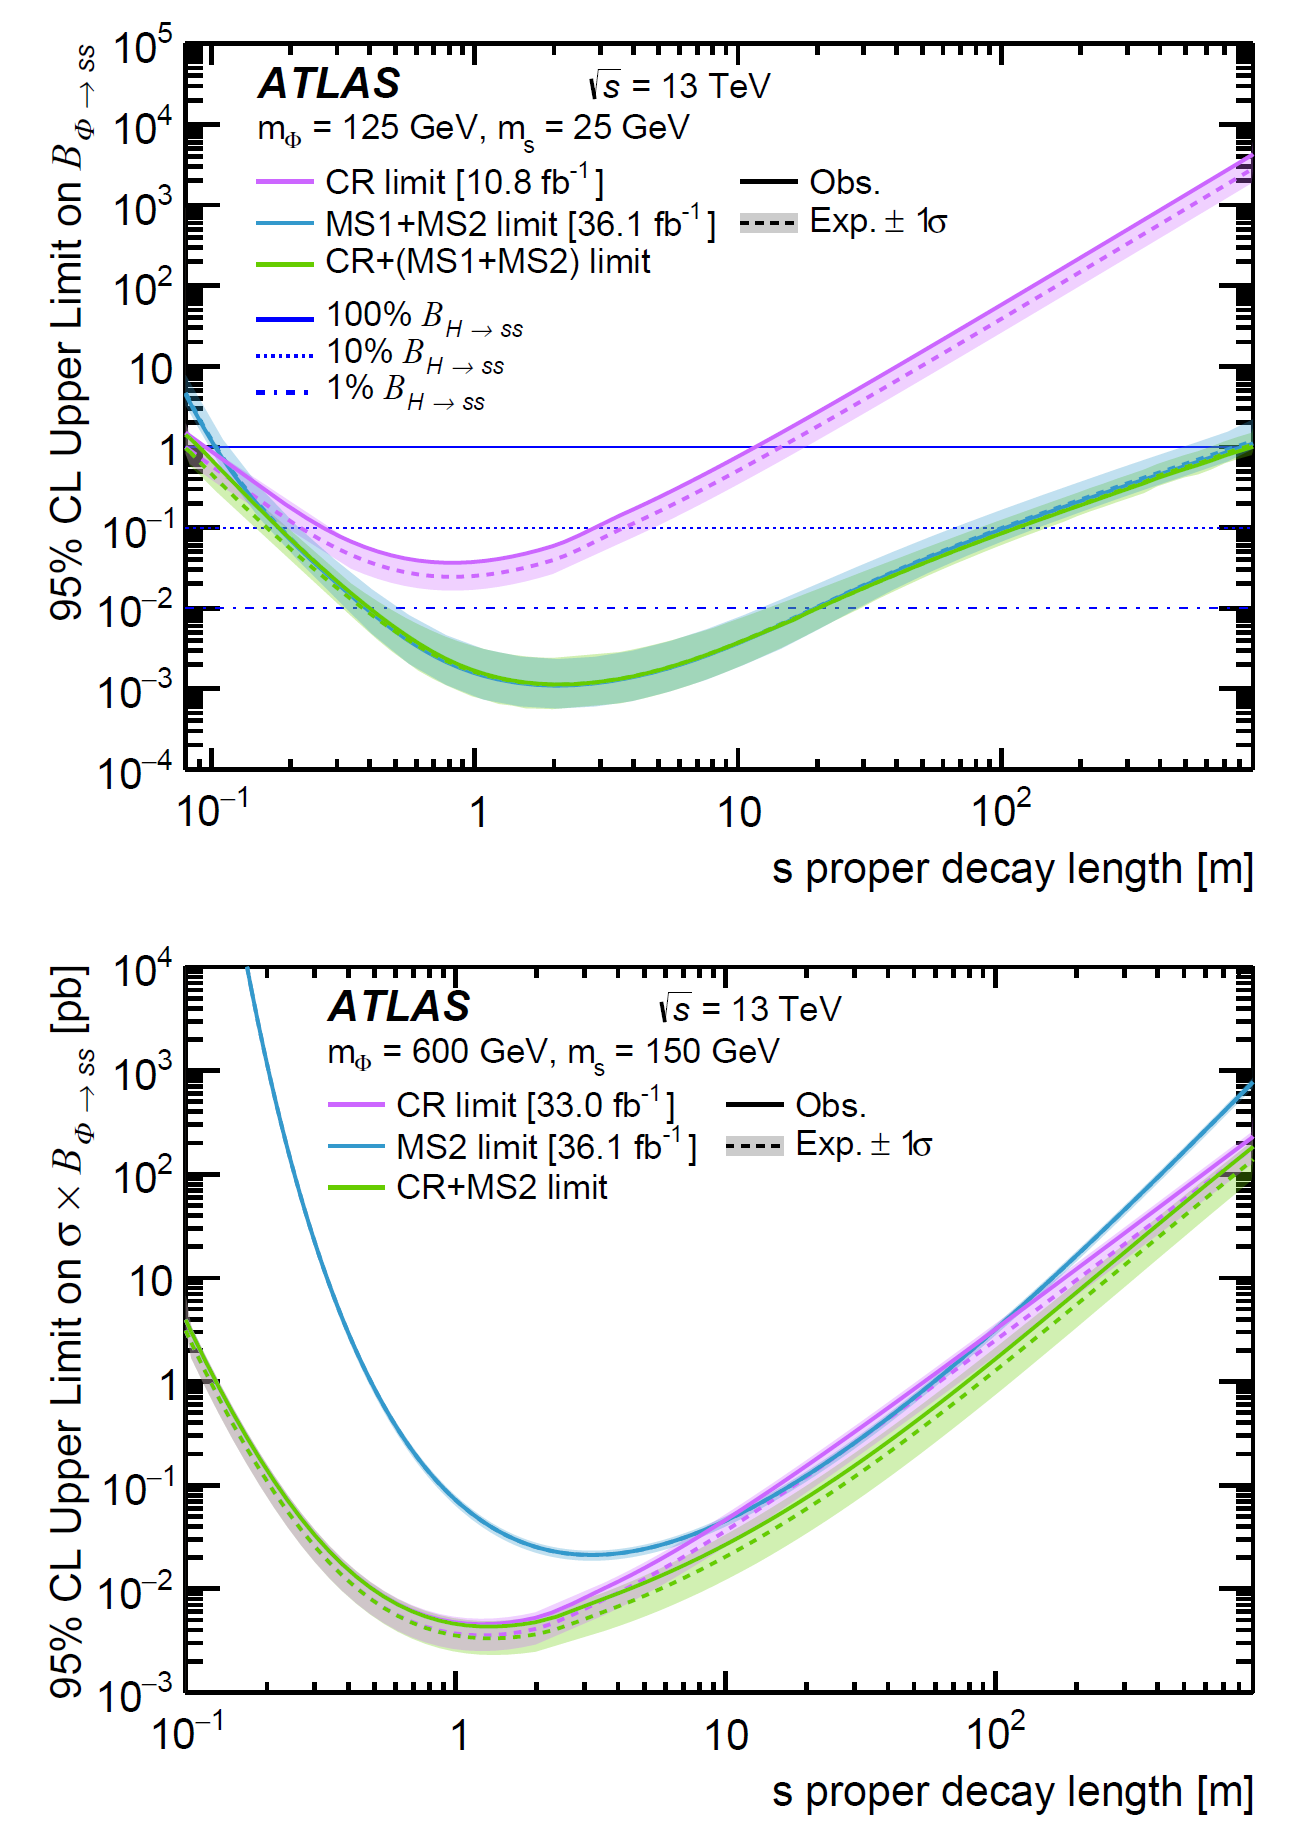
\includegraphics[width=0.5\textwidth]{fig/NeutralLLPinATLAScal.png}
    \label{fig:NeutralLLPinATLAScalSummary}
\end{figure}

\subsubsection{hadronic decay in CMS}

In CMS, the tracking algorithm is based on Kalman filter and can be divided into four steps logically: the \textit{seeding}, in which a proto-track is formed starting from two or three consecutive hits with either a beam spot or a vertex constrain; the \textit{pattern recognition}, during which the proto-trackis propagated into the CMS tracker and compatible hits are associated to the proto-track; the \textit{fitting}, in which the best parameters’ estimate is computed for all hits along the  trajectory; and the \textit{final selection}, in which quality criteria are applied to the tracks to reject the badly reconstructed ones and to reduce the fake rate. This procedure run iteratively, at each iteration, the hits associated to high quality tracks are masked and reduce the complexity of following iterations. During CMS Run \RomanNumeralCaps{2}, ten iterations are deployed with different seedings \cite{CMSPFreconstruction}.
\onecolumngrid
\begin{table*}[!htbp]
    \centering
    \caption{Seeding configuration and targeted tracks of the ten tracking iterations. In the last column, $R$ is the targeted distance between the track production position and the beam axis.}
    \begin{tabular}{cccc}
    \hline
    Iteration  &  Name & Seeding  & Targeted Tracks \\
    \hline
    1  &  InitialStep       &  pixel triplets       & prompt, high $p_T$ \\
    2  &  DetachedTriplet   &  pixel triplets       & from b hadron decays,$R \apprle 5$ cm \\
    3  &  LowPtTriplet      &  pixel triplets       & prompt, low $p_T$ \\
    4  &  PixelPair         &  pixel pairs          & recover high $p_T$ \\
    5  &  MixedTriplet      &  pixel+strip triplets & displaced, $R \apprle 7$ cm \\
    6  &  PixelLess         &  strip triplets/pairs & very displaced,$R \apprle 25$ cm \\
    7  &  TobTec            &  strip triplets/pairs & very displaced,$R \apprle 60$ cm \\
    8  &  JetCoreRegional   &  pixel+strip pairs    & inside high $p_T$  jets   \\
    9  &  MuonSeededInOut   &  muon-tagged tracks   & muons  \\
    10 &  MuonSeededOutIn   &  muon detectors       & muons \\
    \hline
    \end{tabular}
    \label{tab:my_label}
\end{table*}
\twocolumngrid

CMS has inclusive searches for displaced jets using 13 TeV data \cite{Sirunyan:2018vlw,Sirunyan:2018pwn}. The CMS analyses are based on dedicated offline displaced jet tagging algorithm using track information to identify pairs of displaced jets. Displaced tracks associated to each dijet candidate are used to reconstruct a secondary vertex with an adaptive vertex fitter algorithm. Signal preselection criteria require the secondary vertex has $\chi^2/n_dof < 5$, $M_{inv,vertex} > 4$ GeV assuming the pion mass for all assigned tracks and $p_{T,vertex} > 8$ GeV to remove long-lived SM hadrons. In the analysis for 13 TeV data in 2016, an additional variable, $\zeta$, is introduced to characterize the prompt activity to the jet, which is the charged energy fraction of the dijet associated with the most compatible PV. To select the most compatible PV, jet-associated tracks are assigned to primary vertex (PV) if the minimal 3-dimensional impact parameter (IP) significance is less than 5. 

\begin{equation}
\zeta = \frac{\Sigma_{track\in PV_1}E^{Jet_1}_{track}+\Sigma_{track\in PV_2}E^{Jet_2}_{track}}{E^{Jet_1}_{track}+E^{Jet_2}_{track}}
\end{equation}

The triggers used are based on large $H_T = \Sigma |p_{T,j}| = 350 (500)$ GeV for $8 (13)$ TeV, where the $H_T$ sums over jets with $p_{T,j} > 40$ GeV and $|\eta_j| <  3.0$. The signal is interpreted as neutral LLP decaying hardonically and color-charged LLP decaying into a jet plus a lepton. 

For event selection, an auxiliary algorithm is introduced to reveal the consistency of displaced vertex. The displaced tracks associated to dijet are clustered based on the expected transverse decay length with respect to the leading primary vertex $L_{xy}^{exp}$ using a hierarchical clustering algorithm. The cluster root-mean-square (RMS), which is a relative RMS of individual tracks $L_{xy}^{exp}$ with respect to the secondary vertex $L_{xy} $ is computed for signal-background discrimination:

\begin{equation}
    RMS_{cluster} = \sqrt{\frac{1}{N_{tracks}\sigma^{N_{tracks}}_{i=1}}\frac{(L_{xy}^{exp}(i)-L_{xy})^2}{L^2_{xy}}}
\end{equation}

The likelihood discriminant is constructed with vertex track multiplicity, vertex $L_{xy}$ significance and cluster RMS among which the correlations are small. The result for scaler decay $X \rightarrow q\bar{q}$ is shown in Fig. \ref{fig:CMSjetjet}. Results for other models can be found in Ref. \cite{Sirunyan:2018vlw}.

\begin{figure}
    \centering
    \caption{The expected and observed $95\%$ CL upper limits on the pair production cross section of the long-lived particle X, assuming a $100\%$ branching fraction for X to decay to a quark-antiquark pair, shown at different particle X masses and proper decay lengths for the jet-jet model. The solid (dashed) lines represent the observed (median expected) limits. The shaded bands represent the regions containing $68\%$ of the distributions of the expected limits under the background-only hypothesis. From Ref. \cite{Sirunyan:2018vlw}}
    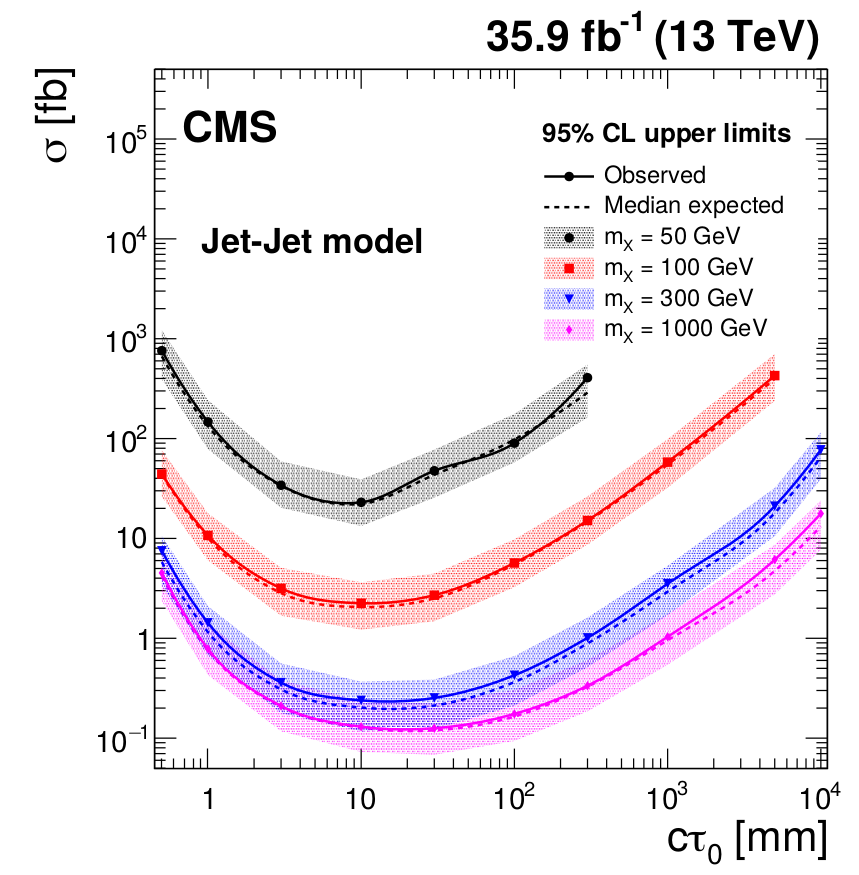
\includegraphics[width=0.5\textwidth]{fig/CMShardonic.png}
    \label{fig:CMSjetjet}
\end{figure}





\subsubsection{hardonic decay in LHCb}
The LHCb is optimized for B physics and use an asymmetric design which make LHCb detector suitable for LLP with shorter time and lower mass. The LHCb searches directly trigger on DV with a transverse distance $L_{xy} > 4mm$ and four or more tracks. The trigger thresholds are low, e.g. the invariant mass of particles associated with the vertex must exceed 2 GeV and the scalar sum $p_T$ of tracks at the vertex must exceed 3 GeV. The jet algorithm is the standard algorithm. The benchmark model used is the decay of scalar into neutral LLP pair, $\pi_{\nu}$ (dark or valley pions) which corresponds to the decay of Higgs/Higgs-like particle. The $\pi_{\nu}$  masses are between 25 and 50 GeV in this search and decay length between 0.6 to 15 mm. LHCb extends the coverage for lower mass LLP with fat jet algorithm and jet  substructure dealing large boosts. Comparison of the ATLAS, CMS and LHCb are made for Higgs simplified model are shown in Fig. \ref{fig:LHCbHadronicCompare}.

\begin{figure}
    \centering
    \caption{Comparison of the ATLAS, CMS and LHCb reaches for dark pions $\pi_{\nu}$ decaying into jets. The CMS result is taken from the recast done the 8 TeV analysi. In the shaded regions $B(H\rightarrow\pi_{\nu}\pi_{\nu})$ is constrained to be below $50\%$. Note that the ATLAS reach extends to higher masses as well; The meaningful bound is on the lifetimes. TFrom Ref.\cite{alimena2019searching}}
    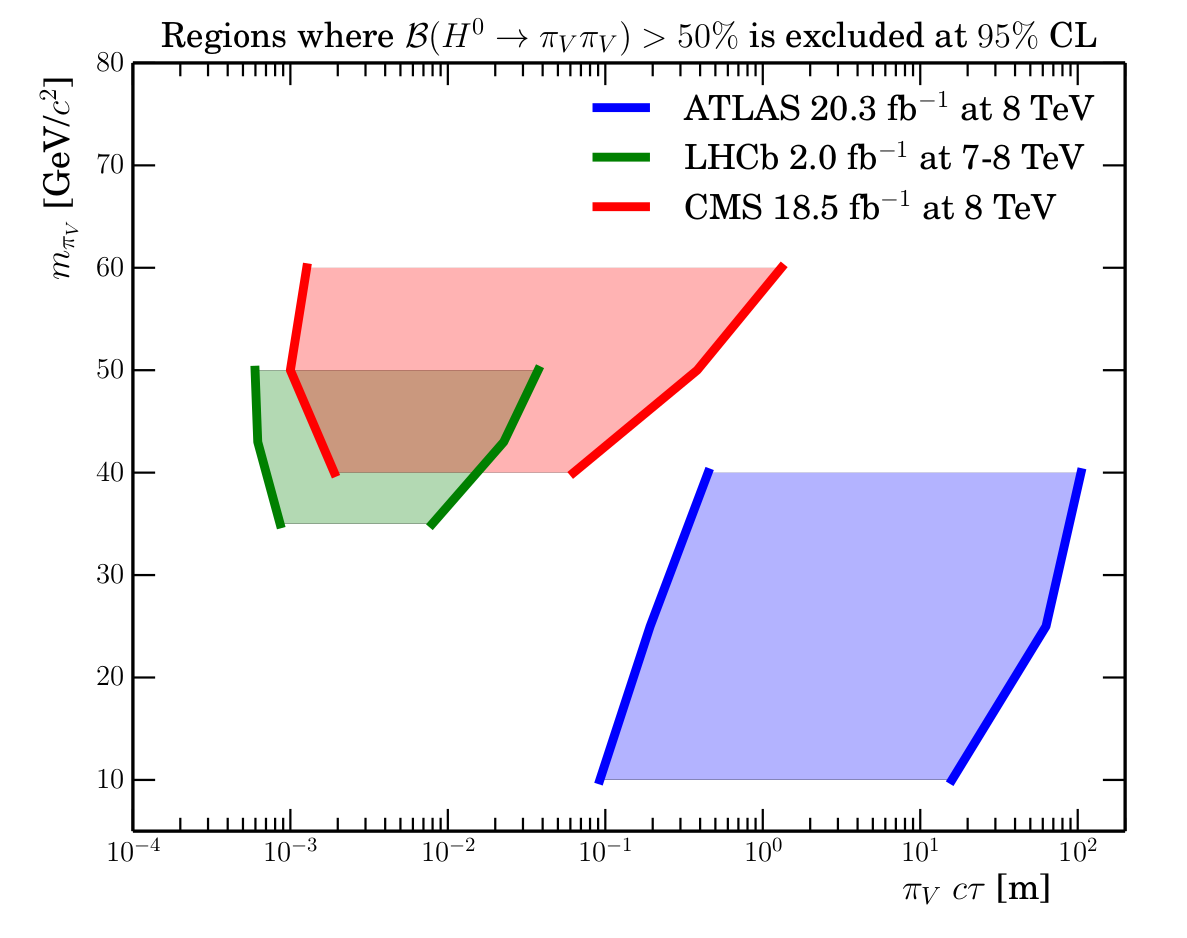
\includegraphics[width=0.5\textwidth]{fig/LHCbhadronicCompare.png}
    \label{fig:LHCbHadronicCompare}
\end{figure}


\subsubsection{summary for hadronic decay}
Current searches with hadronic final states do not cover low mass (<100 GeV) LLP due to the large $p_{T,j}$ trigger requirement with the exception being the DV reconstruction at LHCb. Also, searching strategy in ATLAS require two LLPs decays in detector and lose the sensitivity to singly produced LLP. 

A potential way to extend the coverage of LLP search is to extend the trigger methods and perform the hadronic DV reconstruction offline.Triggering on associated prompt object would improve the sensitivity of low mass LLP significantly.


\subsection{Leptonic Decays}
All three experiments have searches for displaced pair production of leptons. On CMS, dilepton with different flavour and large transverse impact parameter are also searched. Light and boosted LLPs can decay into collimated leptons, known as \textit{lepton-jets}, which are searched in both CMS and ATLAS. The LHCb also search for light. neutral LLPs decaying into muon pair.

\subsubsection{Leptonic decay in CMS}
The CMS tracker-based search trigger on two clustered energy passing loose requirements with photon/electron hypothesis for electron channel and on twp reconstructed muon from muon system without using any PV constraint. The LLP candidates are formed from two opposite-signed muons with $p_T > 26$ or two electrons with higher(lower) $E_T> 40(25)$ GeV. Large transverse impact parameter significance with respect to  PV ( $|d_0|/\sigma_d > 12$) is required for tracks to reject promptly produced particles.  In an complemented research using muon system only, muon candidates are reconstructed from muon system alone. An additional refit step is applied to  the candidates to avoid biases from  a loose beamspot constraint in the seeding step. The candidates then referred as \textit{re-fitted stand-alone} (RSA) muons. Also, the muons are vetoed if they can match to track in the inner tracker. The searches are interpreted in term of SM-like Higgs decay ($H\rightarrow XX, X\rightarrow l^+ l^-$) and RPV squarks and provide sensitivity covering $c\tau$ from $ 10^{-2} (10^{-1})$cm to $ 10^{5} (10^{4})$cm for Higgs (RPV) scenario. The tracker-based search show a high sensitivity plateau with $c\tau \sim 10^{-1}-10$ cm in both electron and muon channels, while the combined result of tracker and muon chamber increases the sensitivity for muon channel with $c\tau > 10$cm. The results are shown in Fig. \ref{fig:LpetonicCMStrackerMuMu} and \ref{fig:LpetonicCMSMSMuMu}.

\begin{figure}
    \centering
    \caption{$95\%$ CL upper limits on $\sigma(H^0\rightarrow XX)B(X \rightarrow \mu^{+} \mu^{−} )$ for $M_{H^0} = 1000 GeV/c^2$ with various X mass points. Shaded bands show the $\pm 1\sigma$ range of variation of the expected $95\%$ CL limits for the case of a $20 GeV/c^2$ X boson mass. From tracker-only search \cite{CMSDiLepton2015}}
    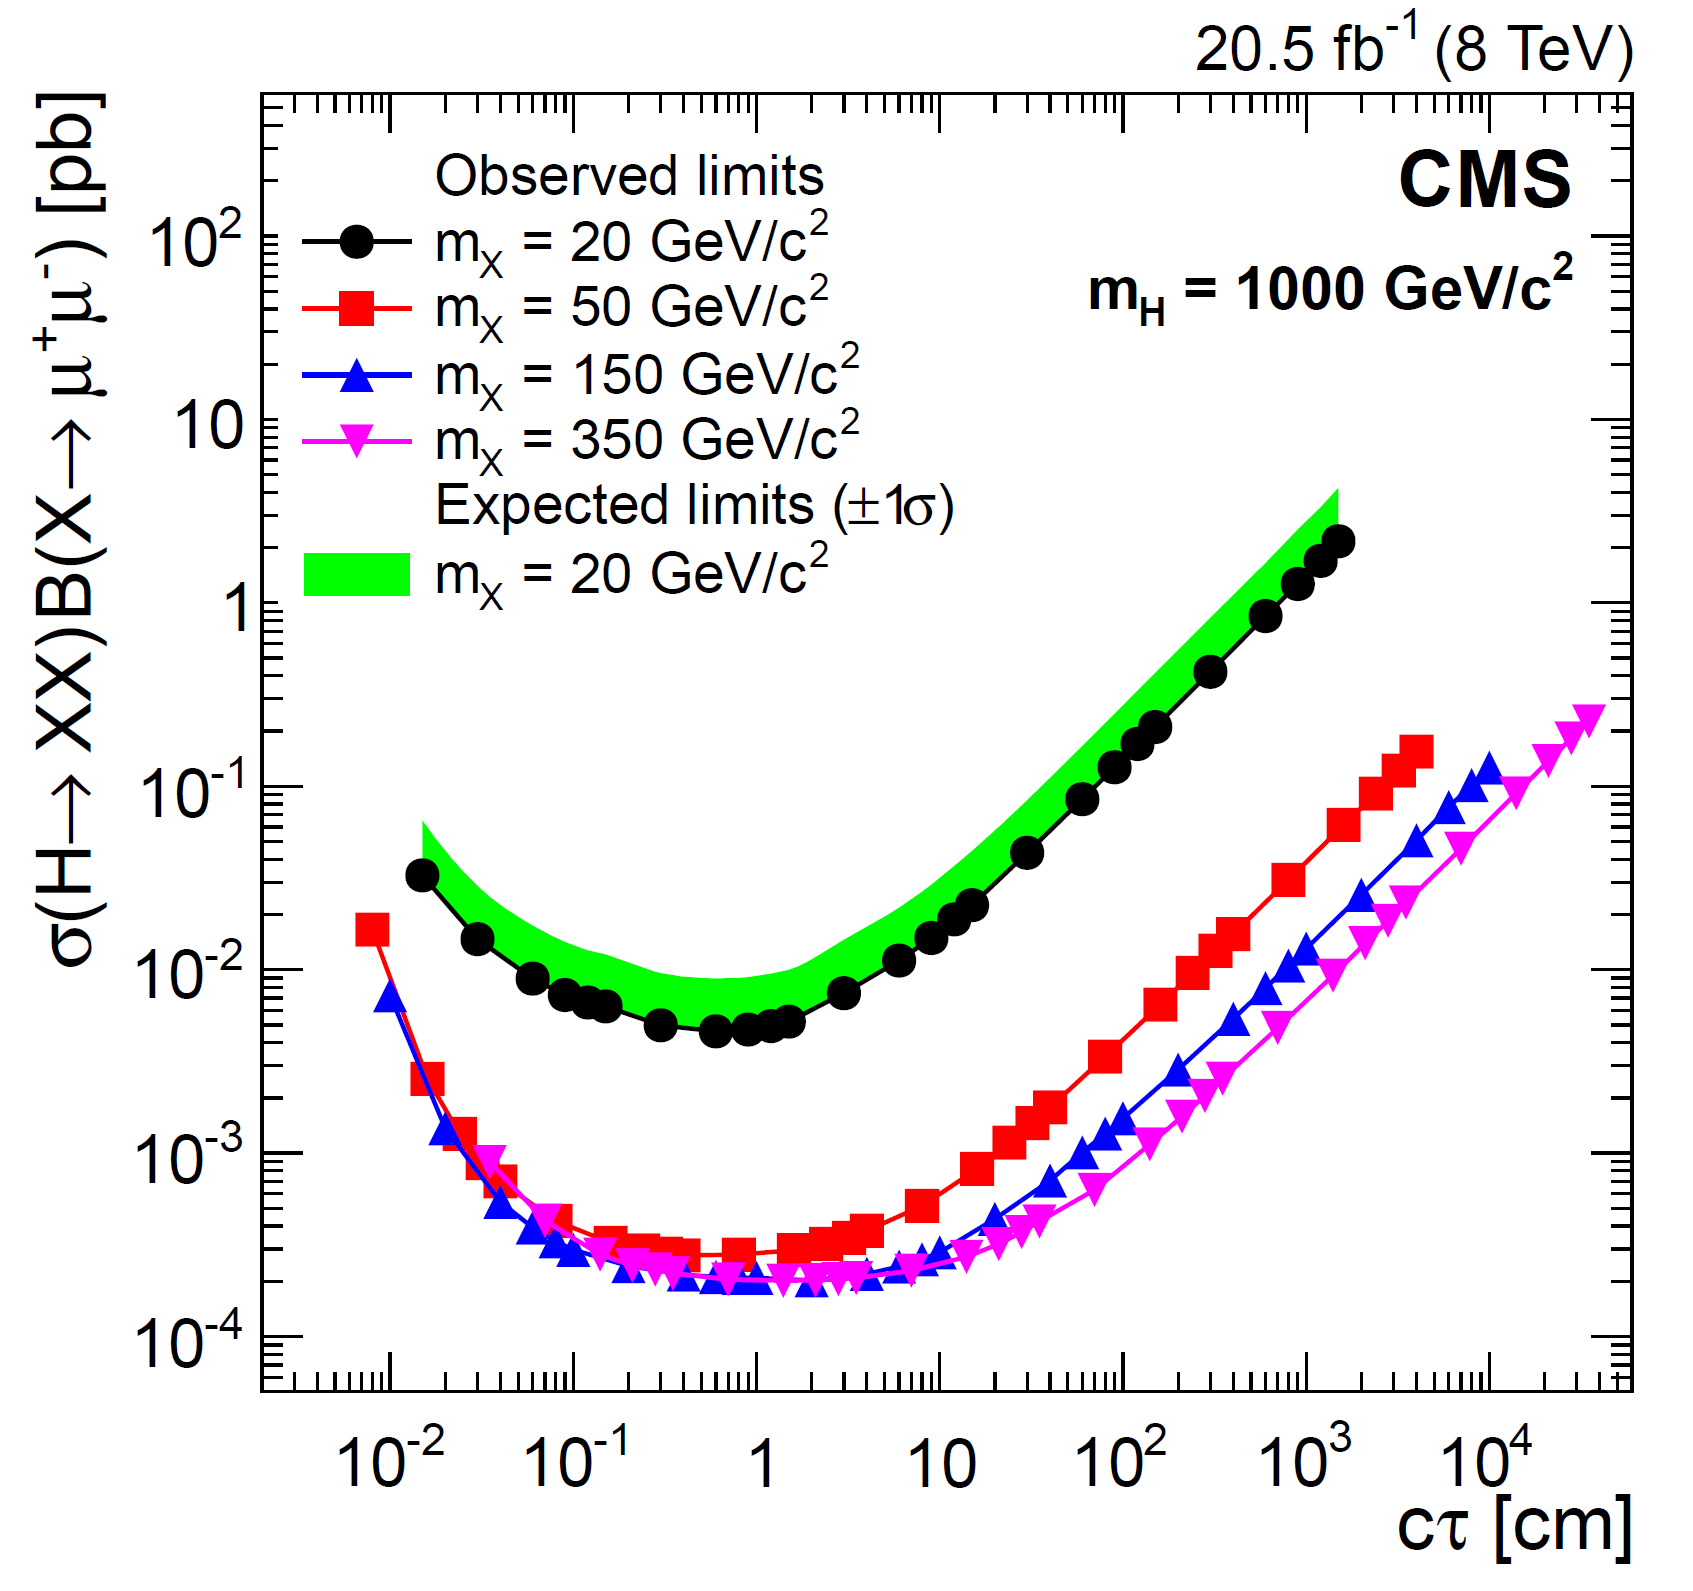
\includegraphics[width=0.5\textwidth]{fig/LpetonicCMStrackerMuMu.png}
    \label{fig:LpetonicCMStrackerMuMu}
\end{figure}

\begin{figure}
    \centering
    \caption{$95\%$ CL upper limits on $\sigma(H^0\rightarrow XX)B(X \rightarrow \mu^{+} \mu^{−} )$ for $M_{H^0} = 1000 GeV/c^2$ with various X mass points. Shaded bands show the $\pm 1\sigma$ range of variation of the expected $95\%$ CL limits for the case of a $20 GeV/c^2$ X boson mass. \cite{CMSDiMuon2015}}
    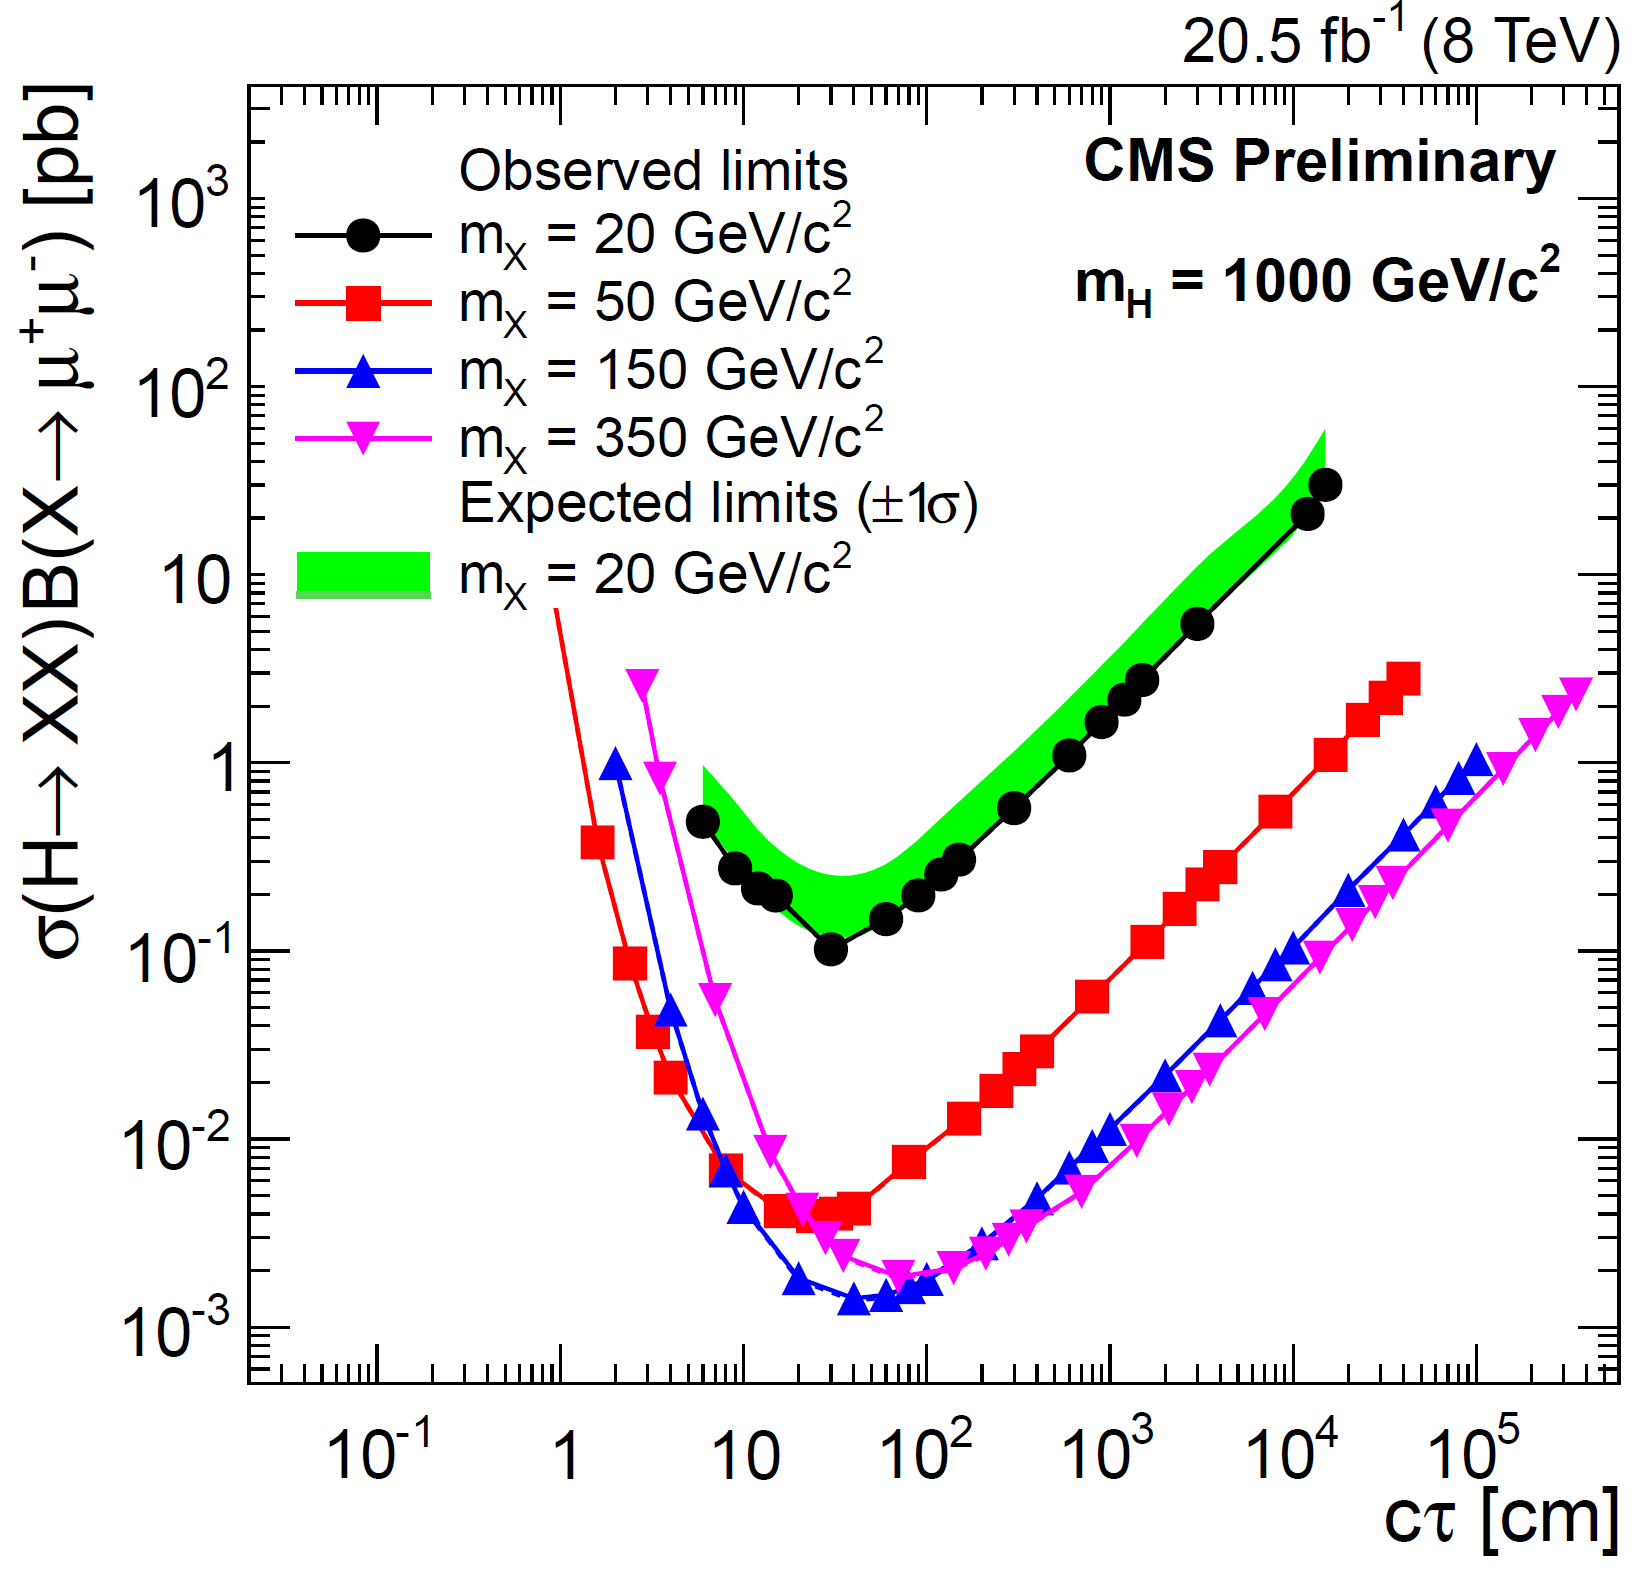
\includegraphics[width=0.5\textwidth]{fig/LpetonicCMSMSMuMu.png}
    \label{fig:LpetonicCMSMSMuMu}
\end{figure}


\subsubsection{Leptonic decay in ATLAS}
 A primary ATLAS search for displaced lepton triggers on muons, electrons or photons. The trigger and offline $p_T$ criteria is relatively high which should pass one of the following: 1). a muon candidate with $p_T > 50$GeV, an electron candidate with $p_T >110$GeV or a photon candidate with $p_T > 130$GeV while the associated ID track are required to have $d_0 > 1.5$mm, 2). a pair of candidate electrons, photons or $e/\gamma$ pair, with $p_T$ threshold between 38 and 48 GeV per object, 3). either two 50 GeV trackless jets with $E_T^{miss} > 100$ GeV or one 45 GeV trackless jets with 4-6 jets passing the same $p_T$ thresholds.  The DV is reconstructed from opposite-sign lepton pair and must be over 4 mm from PV in the transverse plane. DVs in regions with dense detector matter are vetoed to reject backgrounds from converted photons. The high $p_T$ requirement lower the sensitivity of this search to low-mass LLPs.
  A recent search done on ATLAS is using di-muon channel with muon system only, in which four separate trigger pathway are used: $\slashed{E}_T > 110 $GeV; one muon with $p_T > 60$GeV and $|\eta|<1.05$; two muons with $p_T > 15$GeV and $\Delta R_{\mu\mu}<0.5$; or three muons with $p_T > 6$GeV. Thus this search extend the sensitivity to low mass region ($m_{\mu\mu}=15$GeV) as well as with various lepton multiplicities.

\subsubsection{Lepton-jet searches}
Lepton-jets are signature with lepton pair or multiple leptons clustered in a narrow area, which usually originated from the decay of boosted objects. 

In the CMS search for lepton-jet, fully muonic lepton-jets are selected from 8 TeV and part of 13 TeV dataset. The 13 TeV study is sensitive to di-muon parent particle masses up to 8.5 GeV triggered by di-muon with standard isolation requirements. Event selection requires at least four muons, forming two opposite-charged muon pairs in minimum. 

In ATLAS 8TeV search, three types of lepton-jets are considered: only-muon jet, electron/pion jet and inclusive of previous two types. The muon-only and electron/pion jet require two or four leptons while the mixted jet must contain two muons plus a jet consistent displaced with electron/pion pair. The trigger adopted requires three muon tracks in MS with $p_T >$ 6GeV, also the \textit{CalRatio} trigger is used for electron lepton-jet when electrons produced in HCAL. A \textit{narrow-scan} muon trigger is added in 13 Tev analysis. This trigger selects events with two muons close in $\eta-\phi$ plane, $\Delta R < 0.5$ with $p_T > 20(6)$GeV for (sub)leading muon. 

Both the 8 and 13 TeV ATLAS searches are interpreted for Higgs-like scalar particles (with masses of 125 and 800 GeV) that decay effectively into either two or four lepton pairs, with each lepton pair assumed to come from a low-mass “dark" photon, $\gamma_D$ . The ATLAS result excludes exotic Higgs branching ratios below $10\%$ for dark photon lifetimes 2$ < c\tau < $100 mm. Note that here $\gamma_D$ is also allowed to decay to pions and so the results can also be interpreted for hadronically and semi-leptonically decaying LLPs. Also, there are some non-collider experiments constraining the parameter space of $\gamma_D$, which will be discussed in following chapter.
\begin{figure}
    \centering
    \caption{Comparison of the lepton-jet searches at ATLAS, CMS as well as low-energy experiments with respect to a dark photon scenario}
    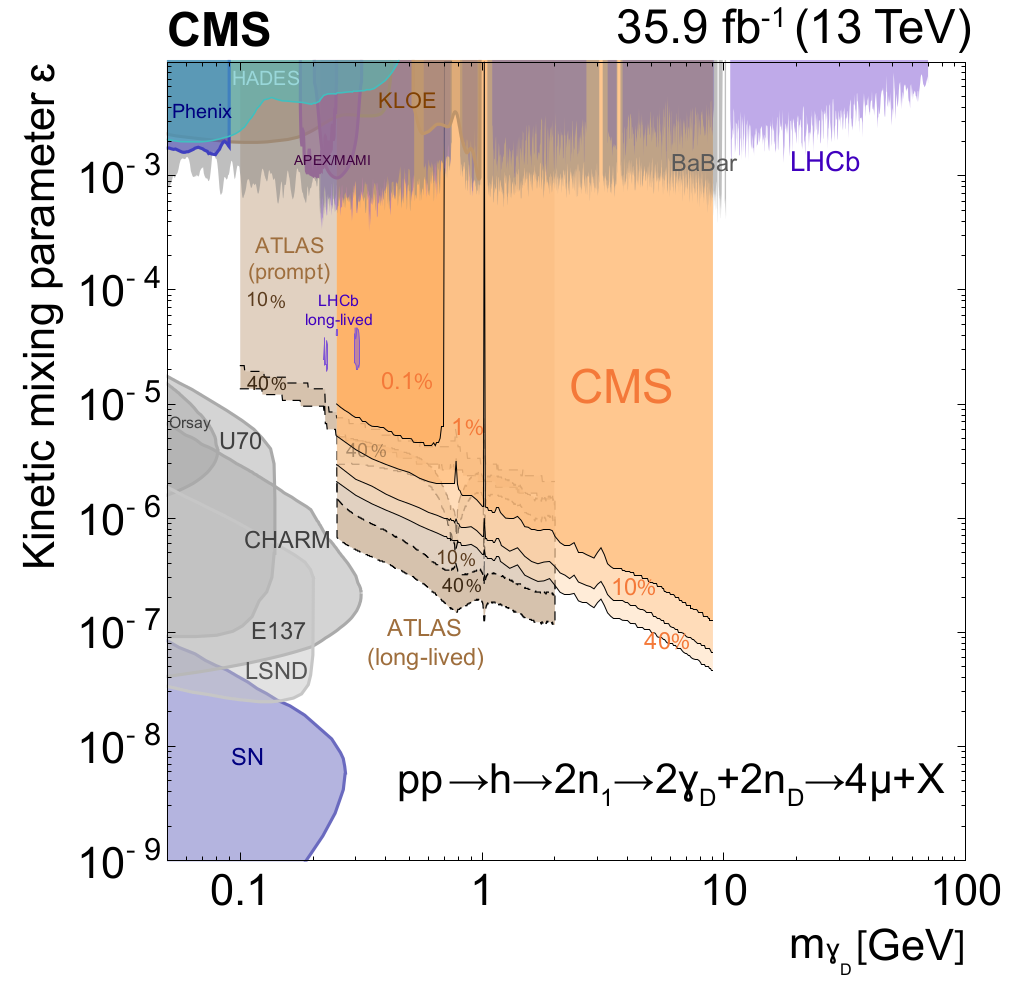
\includegraphics[width=0.5\textwidth]{fig/leptonjet.png}
    \label{fig:lepton-jet}
\end{figure}

The comparison of CMS and ATLAS searches are displayed in Fig. \ref{fig:lepton-jet}.


\subsubsection{Summary for leptonic decay}

The leptonic searches for LLP are based on fairly standard lepton identification and trigger. These searches typically benefit from the low trigger threshold  and good signal efficiency. A major and unavoidable challenge faced by extrapolating the leptonic searches to high-luminosity condition is how to maintain low-threshold trigger for displaced leptons. Another major challenge is coverage of LLP to $\tau$ leptons.Such searches are strongly motivated from theoretical point of view, as higgs-like scalar decays into $\tau^+\tau^-$ dominantly if kinematically permitted. A displaced hadronic $\tau$ is a striking object with few background. Thus the searches with displaced $\tau$s are critical.

\subsection{Semi-leptonic decay}

As semi-leptonic signature shares overlap with both leptonic and hadronic channels, many of the discussed searches are partially covered in this scenario on ATLAS and CMS. LHCb has dedicated searches for semi-leptonically decaying LLPs and semi-leptonic decays of long-lived Majorana neutrinos coming from $B^-$ mesons. 

When applying the inclusive hadronic or leptonic searches to interpret semi-leptonic LLP decay, the simultaneous presence of leptons and jets in the signal can degrade the sensitivity. For instance, the leptonic searches require lepton isolation which significantly reduce the signal acceptance for boosted LLPs decaying leptonically. 

In semi-leptonic LLP searches, one of the major gap is still for low-mass LLPs. The leptons from low-mass LLP have low efficiency to trigger or pass the isolation criteria, background from heavy-flavour and other processes are also higher. The low-mass semi-leptonic LLPs are strongly motivated from Heavy Neutral Leptons (HNL) model, which predicts LLPs for HNLs of masses below 30 GeV. The HNL model corresponds to HNL LLP produced associated with prompt lepton, then decay semi-leptonically into $jjl$.

The sensitivity of LHC experiments to HNLs is complementary to that of fixed-target experiments which can probe lower couplings due to high-intensity beams albeit at lower mass ranges. The projected sensitivity is shown in Fig.\ref{fig:semileptonic}.

\begin{figure}
    \centering
    \caption{Summary of projected experimental sensitivities to HNLs in various experiments, in the coupling strength ($U^2$ for dominant mixing to $\nu_{\mu}$) vs. mass plane.}
    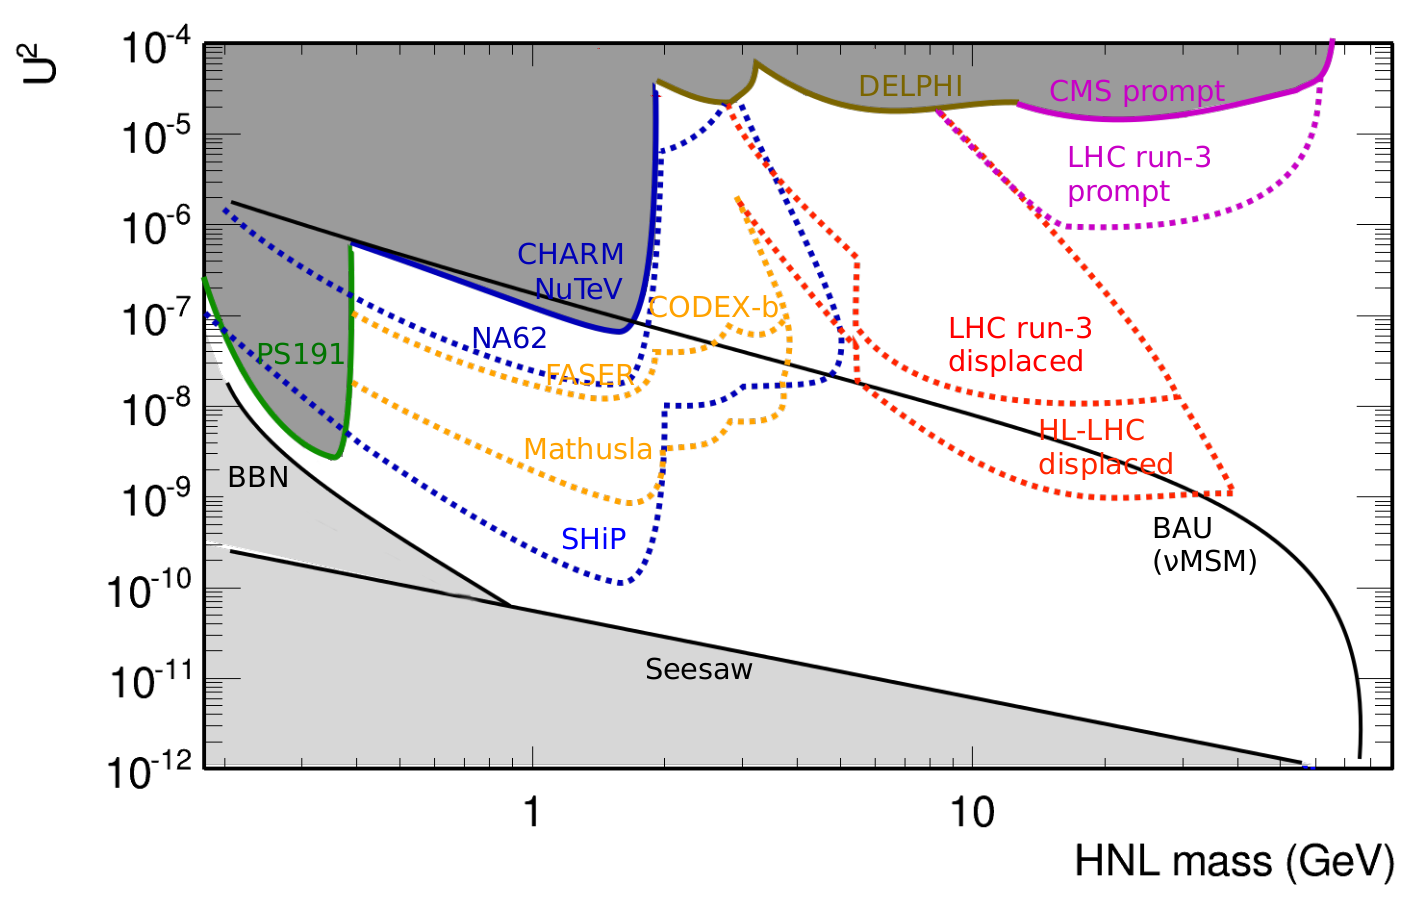
\includegraphics[width=0.5\textwidth]{fig/semileptonic.png}
    \label{fig:semileptonic}
\end{figure}


\subsection{Photonic decay}

As there is no associated track for photon signature, the methods for identifying displaced photon are critical in LLP searches with photonic decay. There are two ways to discriminate photon originating from LLP decay from standard photon. The first is \textit{non-pointing} photon which can not be traced back to PV, and a second one is \textit{delayed} photons when they arrive at the ECAL slower than speed of light. Both signatures are studied at ATLAS with 8 TeV dataset, while on CMS, non-pointing photon are detected via the conversion to $e^+e^-$ pairs. The benchmark model is gauge-mediated supersymmetry breaking (GMSB) in which the neutralino decays into a gravitino and a photon ($\chi^{0}_1 \rightarrow \gamma \tilde{G}$). All searches require large $\slashed{E}_T$ in the final state given the benchmark model. 

\subsubsection{Photonic decay in CMS}

The study of delayed photons on CMS, photons are reconstructed using a clustering algorithm that build a cluster of clusters(supercluster). The supercluster has large size in $\phi$ to recover the efficiency for photons which converted into charged particles and spread by strong magnetic field. The events are triggered by an offline trigger which require at least one isolated ECAL cluster with $E_T$ > 65 GeV and $E_T^miss$ > 25 GeV. Candidate photon are selected from ECAL photon with additional criteria on the shape of cluster. Events are selected if delay time $\delta t$ > 3ns and the timing measurement from multiple crystals are consistence ($\chi^2/nof$ < 4). Furthermore, $\slashed{E}_{T,no \gamma}$ which is the vector sum of $\slashed{E}_T$ and $E_T^{\gamma}$ is used for background discrimination. In signal seletion, both $\slashed{E}_T$ and $\slashed{E}_{T,no \gamma}$ are required to be over 60 GeV.

For non-pointing photon, at least two high $p_T$ isolated photons in association with at least two jets and $E_T^miss$ are required. To identify the displaced photon, $e^+e^-$ pair converted from photon in tracker material are reconstructed. The photon trajectory are then determined from the election pair momentum and vertex with the straight-line assumption of photon. With this method, the reconstructed impact parameter $|d_{XY}|$ of photon adds $40\%$ uncertainty to the signal efficiency.

\subsubsection{Photonic decay in ATLAS}
The ATLAS study benefits from the capability of the liquid-argon eletromagnetic calorimeters to measure the flight direction and the photon's time of flight (TOF). Resolutions on $\Delta z_{\gamma}$, the separation between the PV of the event and the extrapolated origin of the photon, and $|\Delta t_{\gamma}|$, difference of the arrival time of the photon with respect to the prompt case, are as low as 15 mm and 0.25 ns,
respectively. The trigger requires two photons with $E_T$ over 35 and 25 GeV, a PV with 5 or more is required to guarantee the event as $pp$ collision. The summary of the photonic searches on ATLAS and CMS is shown in Fig. \ref{fig:photonicdecay}.

\begin{figure}
    \centering
    \caption{Summary of the $\gamma + \slashed{E}_T$ searches from ATLAS and CMS assuming the same GBSM model. From Ref.\cite{CMSDelayedPhoton}}
    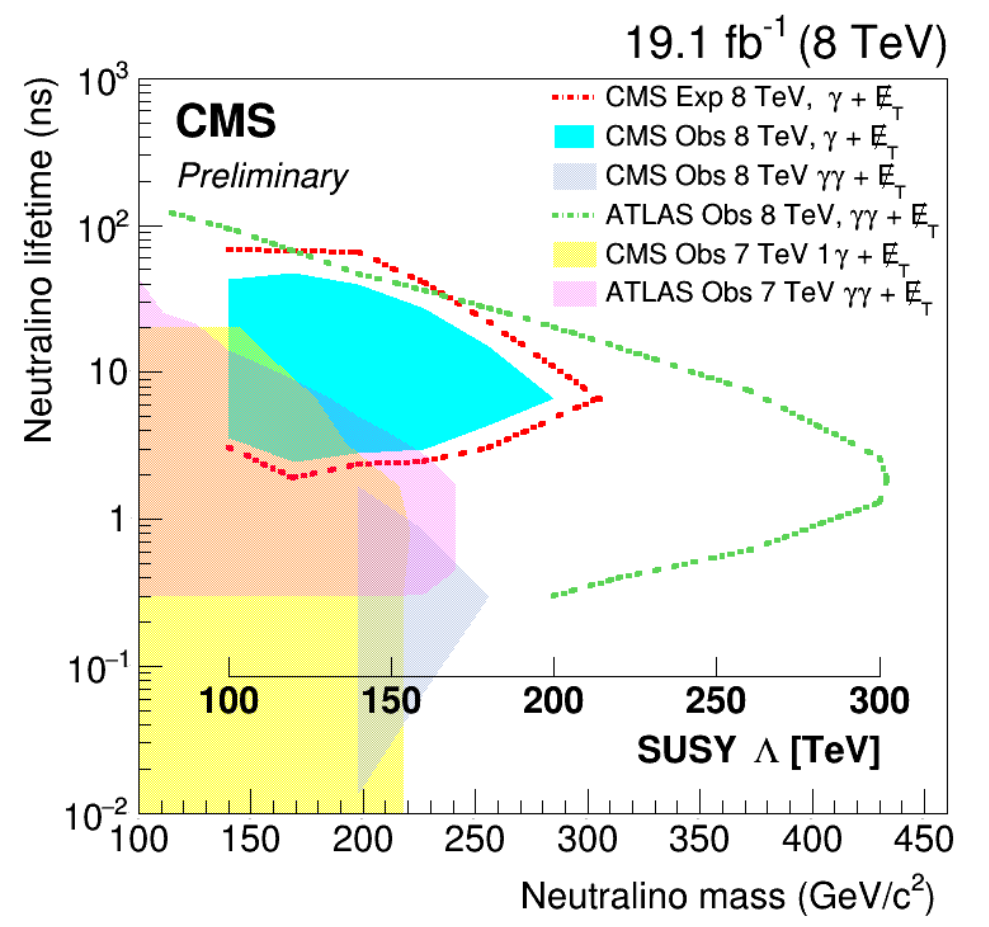
\includegraphics[width=0.5\textwidth]{fig/PhotonicDecay.png}
    \label{fig:photonicdecay}
\end{figure}


\subsubsection{Summary for photonic decay}
In the study on CMS, the identification of displaced photon is the major challenge for non-pointing photon channel which necessitate a development in algorithm. As large $\slashed{E}_T$  is required due to the benchmark model. These searches do not cover the cases without $\slashed{E}_T$, including LLPs that decay to $\gamma\gamma$, $l\gamma$ or $j\gamma$. Also, most searches require two displaced photons while single displaced photon signature is motivated. 

\subsection{Exotic long-lived signature}

Searches for LLP signature with "standard" objects, e.g. jets, leptons and photons are covered in previous sections. While there are still many signatures which are completely distinguished from conventional signatures can be raised by exotic LLPs. These searches are described and summarized in this section, including \textit{disappearing tracks} (DT); \textit{heavy, stable charged particle} (HSCP); \textit{stopped particles} (SP) and monopoles. Other existing ideas searching for LLPs with \textit{quirks} and \textit{Strongly Interacting Massive Particles} (SIMPs) are also described. 

Due to the complexity of exotic signatures, these searches are distinguished into three classes: \textit{LLPs with anomalous geometry}, \textit{LLPs with anomalous interaction} and  \textit{out-of-time decays}. Dedicated event selection are necessary as the trigger as well as  standard reconstruction algorithm have limited efficiency for those exotic signals. 

\subsubsection{LLPs with anomalous geometry}
In this section, LLP signals with anomalous tracking geometry are reviewed. Also, the merging jets signature studied on CMS is included. \\

\textit{Disappearing Tracks(DT)}\\

Massive charge particles traveling in the tracker region can decay into a lighter, almost mass-degenerated neutral particle emitting a soft charged SM particle, e.g. $\pi_{\pm}$ which is hard to be reconstructed in detector. A short track without hits in outer layer of tracker or MS and no associated energy deposit can be reconstructed with standard tracking algorithm, and a charged tracks seems to vanish which referred as disappearing track. The lifetime of charged particle is sensitive to the value of mass splitting as it is constrainted by final state phase space.

Before 2017, both ATLAS and CMS  required a track to travel about 30 cm in order to be reconstructed, giving good coverage of the Wino scenario. This 30 cm value corresponds to four hits at ATLAS, three in the pixel layers plus one in the silicon tracker, and to seven hits in the pixel and trackers of CMS. The search employs a trigger requiring an ISR jet against which the charged particle recoils, along with the presence of large $\slashed{E}_T$. The disappearing track is reconstructed offline and needs to fulfill quality criteria (isolation, $p_T$ threshold, etc.). A phenomenological study has shown that reducing the distance from 30 to 10 cm would give coverage to the elusive Higgsino scenario, moving the expected reach up to 400 GeV, surpassing the expected mono-jet reach of 250 GeV. Later, ATLAS presented a study using 13 TeV data and exploiting the presence of a new innermost pixel layer (IBL). This addition allows for all four hits to be in the pixel, with the outermost pixel layer now at 12.25 cm, enhancing sensitivity to lower values of $c\tau$. CMS also has a disappearing tracks search using 2015 and 2016 data at a center-of-mass energy of 13 TeV which has stronger constraint for $c\tau > 1$ns, shown in Fig. \ref{fig:CMSDisappearingTrack2018}.

\begin{figure}[!htbp]
    \centering
    \caption{The expected and observed constraints on chargino lifetime and mass. The region to the left of the curve is excluded at $95\%$ CL. From \textbf{cite needed}}
    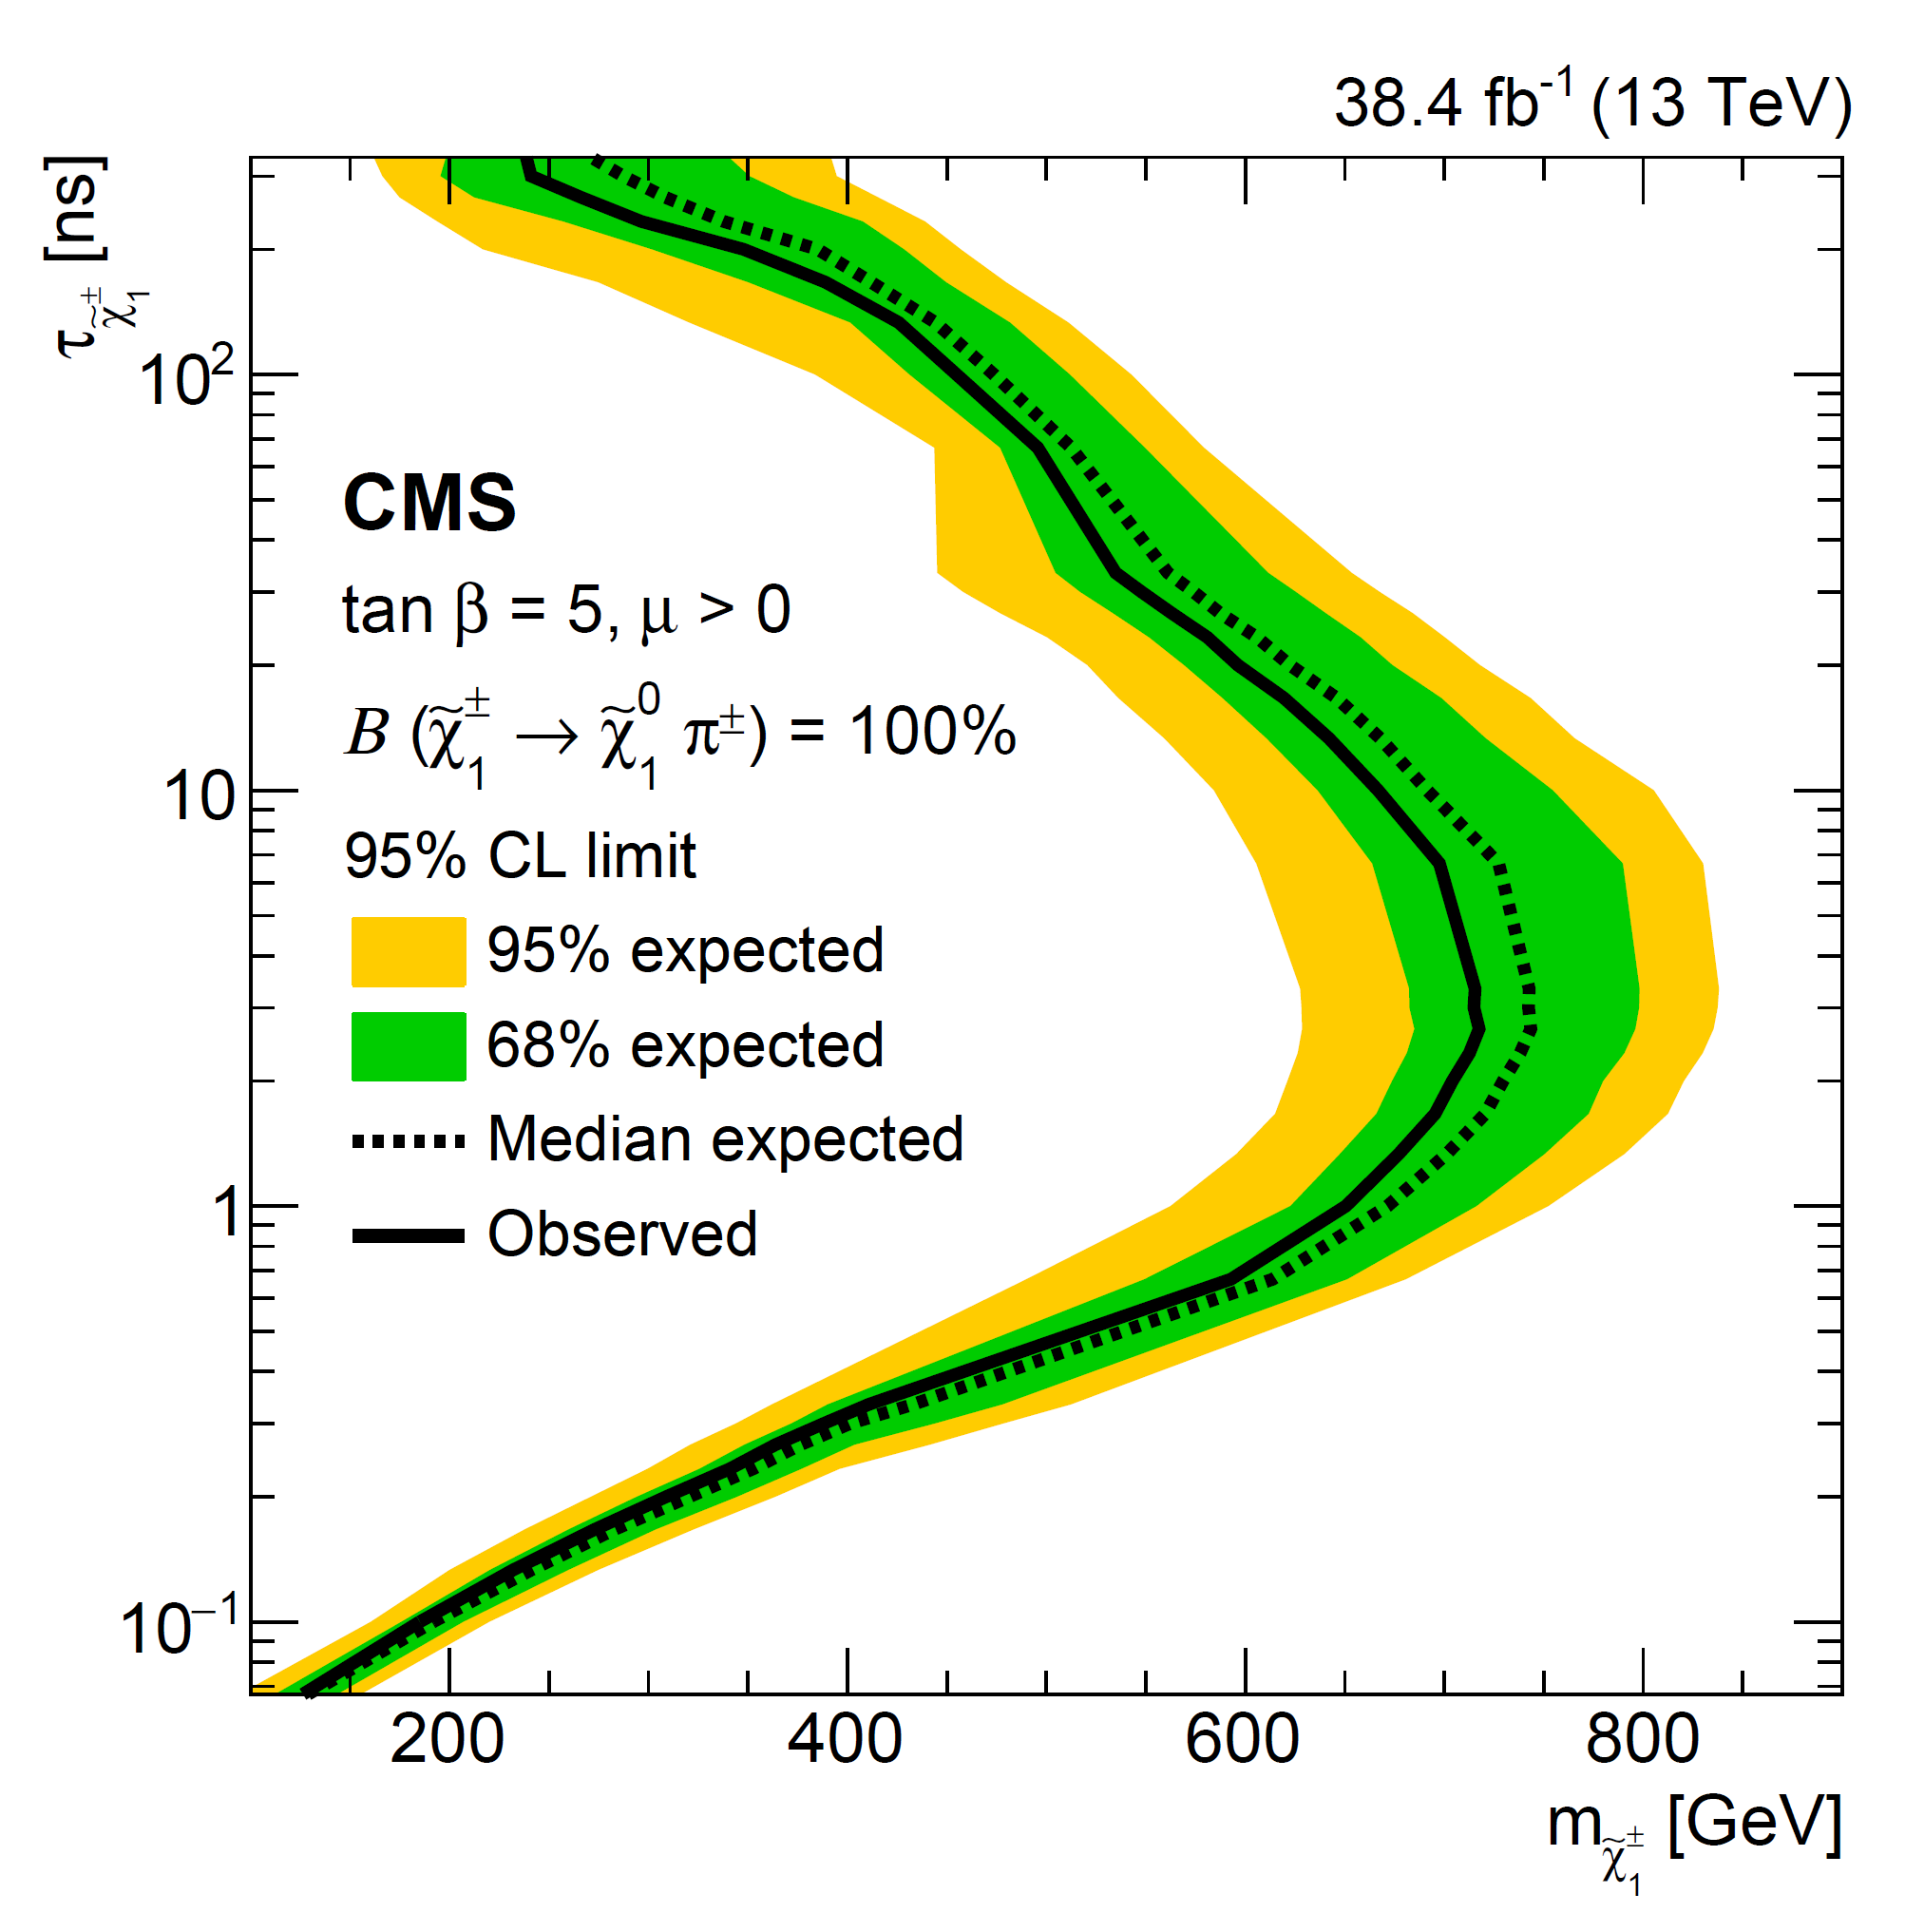
\includegraphics[width=0.5\textwidth]{fig/CMSDisappearingTrack2018.png}
    \label{fig:CMSDisappearingTrack2018}
\end{figure} 

Current searches for disappearing tracks presents a few challenges: using an ISR jet as trigger lower the signal efficiency, Ref.\cite{DisappearingTrackWindow} has shown that significantly lowering the $p_T$ threshold of the jet or directly triggering on the momentum of the disappearing track would lead to a factor of two increase in the number of signal events; extending the sensitivity to lower lifetime is needed, which may only be archived by adding pixel layers closer to interaction vertex or increasing the spatial resolution dramatically. \\


\textit{Quirks}\\

Quirks are electrically charged particle which also color charged under a new confining gauge group, referred to as "infracolor" (IC). The new gauge interaction has confinement scale $\Lambda_{IC} < m_Q$, where $m_Q$ is the mass of quirk. The bound state of quirk-antiquirk is QCD-like system with weak "string" and the constituents are separated by macroscopic distance $l \sim \frac{m_Q}{\Lambda^2_{IC}}$ connected by an infracolor flux tube.

The collider phenomenology depends significantly on the size of $l$, If $l$ is much less than the size of atom, the quirk annihilation take place even before the bound state reaching the beampipe, prompt tracks will be reconstructed. For large enough confinement scales,the infracolor glueball can decay into SM model with large displacement. In some specific case, quirks can produce hidden valley or emerging jet signatures. If the confining force from infracolor charge is weak and $l$ is very large, the constituents behave like heavy stable charged particle (HSCP) which will be discussed in LLPs with anomalous interaction.

A challenging condition of $l$ is to be intermediate and about the size of detector, the confining force will also affect the trajectory of quirk inside the detector. The trjectory of quirk will be bent under both magnetic field and infracolor confining force and be non-helical. For now , there are several theoretical study proposing the search for quirks but there is no public search by the LHC collaborations yet. the lack of constraints on quirks have already attracted the attention of the ATLAS, CMS and LHCb experiments. It would be desirable to test how the phenomenological proposals can perform in a realistic detector simulation of one of the LHC experiments.\\

\textit{Strongly Interacting Massive Particles (SIMPs)}
\\

Strongly interacting massive particles, motivated by astrophysical observation of dark matter which not fully agree with the WIMP paradigm, are assumed to interact strongly with baryons. The experimental signature is then large energy deposit in HCAL with little signal in the tracker and ECAL, which shown as trackless jet. This signature can be triggered by trackless jet associated with a soft muon and the \textit{CalRatio} on ATLAS. A LHC phenomenological study of SIMPs was carried out and proposed an analysis selecting events with high-$p_T$ , back-to-back jets within the tracker, exploiting the charged energy fraction within a jet to discriminate signal from background. The astrophysical experimental constraints on this scenario are compared with the expected reach of this search and that of mono-jets in Fig.\ref{fig:SIMP}.

\begin{figure}
    \centering
    \caption{Astrophysical and collider applicable constraints on a simple SIMP setup. Note that the relevance of the astrophysical constraints depends on the contribution of the SIMPs to the relic density. From Ref.\cite{SimpleSIMP}}
    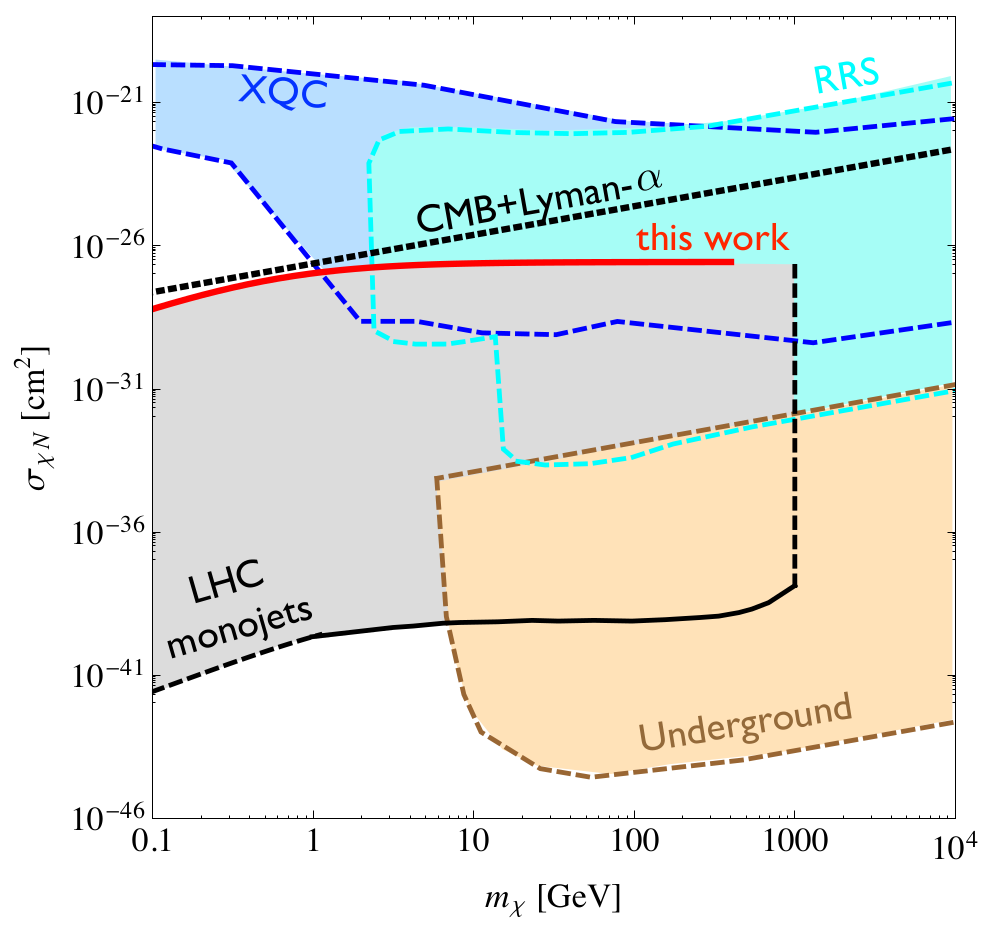
\includegraphics[width=0.5\textwidth]{fig/SIMP.png}
    \label{fig:SIMP}
\end{figure}


\subsubsection{LLPs with anomalous interaction}

In this section, the searches for charged LLPs with anomalous interaction with detector are collected, including heavy, stable charged particles (HSCPs) and magnetic monopoles.\\

\textit{Heavy Stable Charged Particles (HSCPs)}\\

 The researches for HSCP on ATLAS and CMS based on two key properties: particles which is  massive and/or carrying electric charge $|Q| \neq e$ have a characteristic ionization loss ($dE/dx$) distinguishable from SM particles and HSCPs move with $\beta = v/c < 1$ which give rise to a longer time-of-flight (TOF) to reach the outermost component of detector. 

Since the interaction between HSCP with detector can change its electric charge, studies performed on both ATLAS and CMS are separated into \textit{track-only} and \textit{tracker+TOF}. The trigger relies on standard single muon or large MET trigger, the offline selection relies on identifying the signal events from quality requirements on the tracks using discriminator variables built from track observables. In $dE/dx$ maesurement,
 a discriminator $I_as$ is used to distinguish SM particle from HSCP candidate, which defined as:
 
 \begin{equation}
     I_{as} = \frac{3}{N}\times(\frac{1}{12N}+\sum_{i=1}^{N}[P_{i}\times(P_{i}-\frac{2i-1}{2N})^2])
 \end{equation}
 
 where $N$ is the number if measurements in the silicon-tracker detector, $P_i$ is the probability for a minimum-ionizing particle (MIP) to produce a charge smaller or equal to that of the $i$-th measurement for the observed path length in the detector, and the sum is over the track measurements ordered in term of increasing $P_i$. Detailed descriptions for \textit{track-only} and \textit{tracker+TOF} can be found in Ref. \cite{CMSHSCP2016}.

The HSCP search on LHCb is slightly different, which use the lack of radiation emission in the ring imaging Cherenkov detector(RICH) instead of energy loss and TOF. An artificial neural network (ANN) is used to distinguish HSCP from muons by exploitingthe difference in interactions that these particles have in detector. Events are required to pass a high $p_T$ single muon trigger. Two opposite sign muon-like particle are required, each with $p_T$ over 50 GeV and an invariant "dimuon" mass above 100 GeV to suppress muon events from Drell-Yan process.
 
The theoretical interpretation of a signal depends on the type of charge carried. If the HSCP carries a color charge, the benchmarks correspond to $R$-hadron which hadronize into SM particles via the strong interaction. In the absence of a color charge, the signal is interpreted by long-lived sleptons in the context of gauge-mediated SUSY. Both scenarios are employed in ATLAS and CMS studies while LHCb uses a stau benchmark model.  Also CMS looks for HSCPs coupling only to hypercharge and ATLAS has a study for associated production of a neutral and an electrically charged LLP, which is one HSCP with large missing energy. 

To summarize, HSCP searches employ standard trigger and tracking algorithm  and the analysis methods are well-understood and validated by existing searches. However, milli-charge particles are not covered as the ionization in tracker system is tiny and  dedicated detectors, e.g. MilliQan, are proposed.\\

\textit{Magnetic Monopoles}\\

Magnetic monopole is predicted to explain the quantization of electric charge. The main phenomenological feature is that magnetic mnopole is highly ionizing particle (HIP) which hehaves like a particle carrying 68.5 electric charges. A dedicated searches for HIPs use trigger based on identifying relevant \textit{RoIs} in the ECAL and subsequently counting the number of hits in the transition radiation tracker (TRT). The fraction of TRT hits with ionization larger than $\sim 3$ times that expected from a SM particle is used as a discriminant. The event selection is based on the fraction of TRT-HT hits matched to an EM cluster deposit, and how the energy deposits are distributed in the different layers of the ECAL. 


\subsubsection{Out-of-Time Decays of stopped particle}

An unique signature of LLP is out-of-time decay when particles produce out of the collision time window. The only member of this class is the search of stopped particles (SP). For LLPs produced with low kinetic energy, they can lose all the kinetic energy through interaction with detector materials and stop inside the detector, most likely in the calorimeters or the steel yoke in the muon system as a result of their high material densities. The LLPs then decay later when no collision is taking place at beam spot. 

Analysis are performed in ATLAS and CMS with Run I dataset. The events are selected with dedicated trigger selecting bunch crossings away from in-time collisions. The offline selection procedure is aimed at reducing the main backgrounds: cosmic muons, beam halo and instrumental noise. Muons from cosmic rays can be identified with distinctive topology and time structure. The "beam halo" background comes from the interaction between proton and pipeline/collimators, the produced muon travel parallel to the beam and leave energy deposit in calorimeter after a long time-of-flight. Instrumental noise is rejected in CMS by a series of offline criteria that exploit these timing and topological characteristics to remove spurious events due to noise.



% Insert non-Collider Experiments for LLP
\section{Constraints from Non-collider Searches}



% Insert Dedicated Detectors in Future
\section{Dedicated Detectors in Future}

Despite a various of researches are done or proposed with superficially comprehensive coverage of LLP at the LHC, there are still cases, including ultra-low-mass particle, ultra-long lifetime particle and , which are barely covered by main experiments at LHC, due to the difficulties in triggering, object reconstruction and event selection. Hence, new proposals for dedicated experiments for LLPs are put forward to fill in these missing pieces. These new experiments are expected to provide good sensitivity to millicharged LLPs, magnetic monopoles and other LLPs hard to trigger or reconstructed.

In general, high mass LLPs with high $p_T$ final states are covered with excellent sensitivity on ATLAS and CMS. Low mass LLPs are more challenging with higher backgrounds and low selection capability of triggers. In the short time regime, as the $c\tau$ comparable with the scale of VErtex LOcator (VELO), the sensitivity extends to lower mass in LHCb. For low-mass LLPs with long-lifetime, few sensitivity can be archived in majar experiments at LHC. LLPs with weak ionization, e.g. millicharged partcle, are barely visible in ATLAS, CMS and LHCb. These signatures can be covered by NA62 operating in beam dump mode, or by dedicated LHC experiments like milliQan, CODEX-b, FASER, or MATHUSLA. Each of dedicated experiments are sensitive to specific type of LLP signature.

\subsection{The milliQan Experiment}

MilliQan is a proposed dedicated experiment conducted at the LHC targeting non-quantized charged particle referred to as \textit{milli-charged particle} (mCP). The milliQan experiment is a segment of a general program to search for hidden sectors and other BSM scenarios. To estimate the potential reach of milliQan from theoretical aspect, an appealing example is built with an extra abelian gauge field added into the SM model. The additional gauge field couples to a massive Dirac fermion ("dark QED") and mixes with hypercharge through the kinetic term:
\begin{equation}
\mathcal{L} = \mathcal{L}_{SM}-\frac{1}{4}A_{\mu\nu}^{'}A^{'\mu\nu}+i\bar{\psi}(\slashed{\partial}+ie^{'}\slashed{A}^{'}+ iM_{mCP})\psi-\frac{\kappa}{2}A^{'}_{\mu\nu}B^{\mu\nu}
\end{equation}
Eliminating the mixing term by redefining the new gauge boson as $A_{\mu}^{'}\rightarrow A_{\mu}^{'} + \kappa B_{\mu}$, the coupling of massive charged particle to hypercharge shown as 
\begin{equation}
\mathcal{L} = \mathcal{L}_{SM}-\frac{1}{4}A_{\mu\nu}^{'}A^{'\mu\nu}+i\bar{\psi}(\slashed{\partial}+ie^{'}\slashed{A}^{'} - i\kappa e^{'}\slashed{B}+ iM_{mCP})\psi
\end{equation}
The new fermion field $\psi$ acts as particle carrying a milli-charge $\kappa e^'$, the mCP $\psi$ couples to the photon and Z boson with a charge $\kappa e^{'}\cos{\theta_W}$ and $-\kappa e^{'}\sin{\theta_W}$. The fractional charge in unit of the electric charge is $\eposilon \equiv \kappa e^' \cos{\theta_W}/e$



% Insert Summary
\section{Summary}



\appendix



% The \nocite command causes all entries in a bibliography to be printed out
% whether or not they are actually referenced in the text. This is appropriate
% for the sample file to show the different styles of references, but authors
% most likely will not want to use it.
\nocite{*}

\bibliography{LLP}% Produces the bibliography via BibTeX.

\end{document}
%
% ****** End of file apssamp.tex ******
